\documentclass[12pt, a4paper]{report}

\usepackage[czech]{babel}
\usepackage[utf8]{inputenc}
%\usepackage[cp1250]{inputenc}
\usepackage[IL2]{fontenc}
%\usepackage{anyfontsize}
\usepackage{graphicx}
\usepackage{float}
%\usepackage{pdfpages}

\title{Tabletová aplikace pro jednotku intenzivní péče}
\author{David Pivovar A13B0403P}

%%%%%%%%%%%%%%%%%%%%%%%%%%%%%%%%%%%%%%%%%%%%%%%%%%%%%%%%%%%
%%%%%Makra%%%%%%%%%%%%%%%%%%%%%%%%%%%%%%%%%%%%%%%%%%%%%%%%%

% Tato makra přesvědčují mírně ošklivým trikem LaTeX, aby hlavičky kapitol
% sázel příčetněji a nevynechával nad nimi spoustu místa. Směle ignorujte.
\makeatletter
\def\@makechapterhead#1{
  {\parindent \z@ \raggedright \normalfont
   \Huge\bfseries \thechapter. #1
   \par\nobreak
   \vskip 20\p@
}}
\def\@makeschapterhead#1{
  {\parindent \z@ \raggedright \normalfont
   \Huge\bfseries #1
   \par\nobreak
   \vskip 20\p@
}}
\makeatother

% Toto makro definuje kapitolu, která není očíslovaná, ale je uvedena v obsahu.
\def\chapwithtoc#1{
\chapter*{#1}
\addcontentsline{toc}{chapter}{#1}
}



%%%%%%%%%%%%%%%%%%%%%%%%%%%%%%%%%%%%%%%%%%%%%%%%%%%%%%%%%%%
%%%%%Zacatek dokumentu%%%%%%%%%%%%%%%%%%%%%%%%%%%%%%%%%%%%%

\begin{document}

%%%%%%%%%%%%%%%%%%%%%%%%%%%%%%%%%%%%%%%%%%%%%%%%%%%%%%%%%%%
%%%%%Titulni strana%%%%%%%%%%%%%%%%%%%%%%%%%%%%%%%%%%%%%%%%
\begin{titlepage}

\begin{center}
	
	{\fontsize{22}{0} \selectfont
		Západočeská univerzita v Plzni\\
		Fakulta aplikovanch věd\\
		Katedra informatiky a výpočetní techniky\\
	}
	
	\vfill
	\vfill
	
	{\fontsize{28}{0} \textbf{
		Bakalářská práce\\
	}}
	
	\vfill
	
	{\fontsize{36}{0} \textbf{
		Tabletová aplikace\\pro jednotku intenzivní péče
	}}

\end{center}

\vfill
\vfill
\vfill
\vfill

\begin{flushleft}

	{\fontsize{16}{0} \selectfont
		Plzeň, 2016
		\hfill
		David Pivovar
	}
	
\end{flushleft}

\end{titlepage}

%%%%%%%%%%%%%%%%%%%%%%%%%%%%%%%%%%%%%%%%%%%%%%%%%%%%%%%%%%%
%%%%%Kapitoly%%%%%%%%%%%%%%%%%%%%%%%%%%%%%%%%%%%%%%%%%%%%%%

%\setlength{\parskip}{1em}
%\begin{abstract}
\section*{Abstract}
MediTab is a tablet information system designed for nurses to manage patient records. It replaces printed form of records. It allows instant access to data in the database and makes the process of transferring and storing of new actual data more effective. Application complements desktop application WinMedicalc (Medicalc software s. r. o.).
%\end{abstract}

\vfill

%\begin{abstract}
\section*{Abstrakt}
MediTab je tabletový informační systém určený zdravotním sestrám pro správu záznamů o pacientech. Nahrazuje tištěnou formu záznamů o pacientech. Umožňuje tak okamžitý přístup k datům v databázi a zefektivňuje proces přenosu a ukládání nových aktuálních dat.Aplikace doplňuje desktopovou aplikaci WinMedicalc (Medicalc software s. r. o.).
%\end{abstract}

\vfill

\tableofcontents

\setlength{\parskip}{1em}
\chapter*{Úvod}
\addcontentsline{toc}{chapter}{Úvod}

Předmětem této práce je vytvořit grafické uživatelské rozhraní tabletové aplikace pro jednotku intenzivní péče ve Fakultní nemocnici v Plzni. Tato aplikace je určena především pro zdravotní sestry. Na nemocničním pokoji bude k dispozici tablet s aplikací, kde zdravotní sestra bude mít k dispozici aktuální data o pacientech a bude do aplikace zanamenávat své provedené úkony.

Aplikace nahradí tištěnou formu medikačních záznamů a záznamů o pacientech. Umožní tak okamžitý přístup k datům v databázi a zefektivní proces přenosu a ukládání nových aktuálních dat. Aplikace zefektivní práci jak zdravotních sester, tak i lékařů. Každý provedený úkon zdravotní sestrou se okamžitě promítne do databáze a lékař ho uvidí na svém PC. Díky propojení dat s databází se předejde ručnímu přepisování, při kterém se zvyšuje chybovost.

Cílem je vytvořit jednoduché a intuitivní uživatelské rozhraní, které se podobá zavedeným postupům ve FN Plzeň. Vzorem pro vývoj tabletové aplikace je desktopová aplikace WinMedicalc vyvíjená plzeňskou firmou Medicalc software s.r.o. ve spolupráci se SIS FN Plzeň\footnote{Správa informačního systému (IT oddělení nemocnice)}.

Tabletovou aplikaci pro jednotku intenzivní péče jsem nazval pracovním názvem \emph{MediTab}.

V první časti této práce je popsáno prostředí jednotky intenzivní péče nemocnice a aplikace WinMedicalc, části, které jsou společné s vyvíjenou aplikací (kapitola \ref{ch:fn}). Druhá část se zabývá požadavky na vyvíjenou aplikaci (kapitola \ref{ch:specifikace}) a jejím návrhem (kapitola \ref{ch:navrh}). V poslední části je popsána implementace uživatelského rozhraní (kapitola \ref{ch:implementace}) a průběh testování aplikace (kapitola \ref{ch:test}).
\setlength{\parskip}{1em}
\setlength{\parskip}{1em}

\chapter{Prostředí FN Plzeň}

Tato kapitola se zabývá obecným popisem prostředí jednotky intenzivní péče ve FN Plzeň, databáze ve FN Plzeň a aplikace WinMedicalc - karet \emph{Ordinované léky}, \emph{Bilance tekutin} a \emph{Invazivní přístupy}.

\section{Práce zdravotních sester}

Práce zdravotních sester v nemocnici je náročná a vyžaduje zodpovědnost. Sestry musí být pečlivé a nedělat chyby, které by mohli ohrozit zdravotní stav pacienta. Obvzlášť tomu je na jednotkách intenzivní péče, kde musí rychle reagovat na změny stavu pacientů. Tomu musí být přizpůsobená i vyvíjená aplikace. Její ovládání musí být jednoduché a intuitivní, aby práce s ní byla efektivní.

Zdravotní sestry na jednotce intenzivní péče často pracují v latexových rukavicích. Tomu by mělo odpovídat i uživatelské rozhraní. Jednotlivé komponenty by měly proto být dostatečně veliké, aby nedocházelo ke zbytečným překlepům. Je třeba počítat i s tím, že některá zdravotní sestra může mít zrakovou vadu. Neustálé nasazování brýlí by ji poté zdržovalo od práce. Také proto je nutné použít dostatečně velké komponenty a písmo.

Způsob práce a zápisu dat se na jednotlivých odděleních nemocnice liší dle jejich zvyklostí. Proto je nutné udržovat data v konzistentní formě. K tomu ve FN Plzeň slouží program WinMedicalc.

\section{WinMedicalc}

WinMedicalc je nemocniční informační systém, který usnadňuje a zrychluje vytváření lékařské dokumentace. Dále zajišťuje vykazování zdravotní péče a uchovávání dat v jednotné struktuře. Také obsahuje nástroje z oblasti managementu.

Každý pracovník FN Plzeň je v nemocniční databázi. Na základě vlastního uživatelského jména a hesla má přístup do aplikace WinMedicalc s povolenými funkcemi vzhledem k jeho pracovní pozici.

\subsection{Ordinované léky}

Karta ordinovaných léků slouží k evidenci podávaných léků u pacienta. Lékař zde zadává léky, které se pacientovi mají podávat. Ke každému léku doplňje množství, kolikrát denně a od kdy do kdy se má lék podávat (viz obrázek \ref{fig:WM_ordinovane_leky}).

\begin{figure}[H]
	\centering
	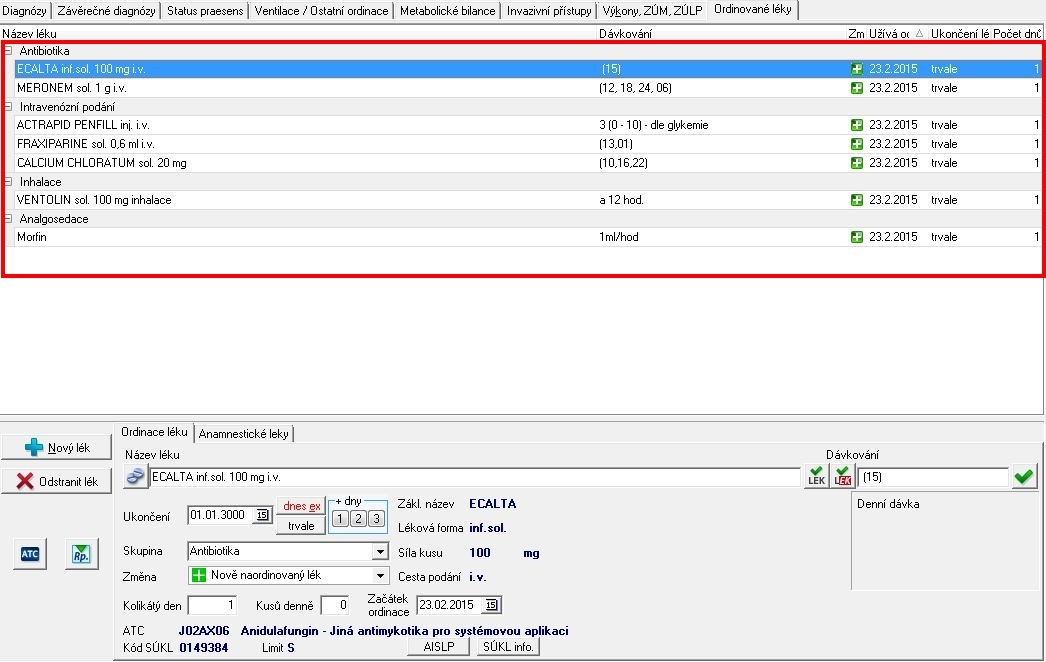
\includegraphics[width=1\textwidth]{img/medicalc/WM_ordinovane_leky.eps}
	\caption{Ordinované léky (WinMedicalc)}
  \label{fig:WM_ordinovane_leky}
\end{figure}

Medikační karta pro každého pacienta se poté vytiskne na papír do tabulky s vyznačenými hodinami. Tabulka nezačíná od půlnoci, ale od hodiny, kterou mají na oddělení nastavenou jako začátek dne (obvykle to bývá 6-7 hodina). Zdravotní sestry poté podle medikační karty podávají předepsané léky jednotlivým pacientům.

Medikační kartu musí vždy před vytištěním schválit lékař. Pokud to nestihne do začátku dne, vytiskne se karta z předchozího dne. Zdravotní sestry pak podávají léky podle této karty do doby, než se schválí a vytiskne nová medikační karta. Překrývající se údaje poté přepíší.

\subsection{Bilance tekutin}

V bilanci tekutin se zaznamenává příjem a výdej veškerých tekutin pacienta na lůžku i na operačním sále za celý den. Zaznamenává se 7 tekutin pro příjem a 5 tekutin pro výdej. Zároveň se počítá celkový příjem a celkový výdej všech tekutin. Rozložení jednotlivých tekutin je vidět na obrázku \ref{fig:WM_bilance_tekutin}.

\begin{figure}[H]
	\centering
	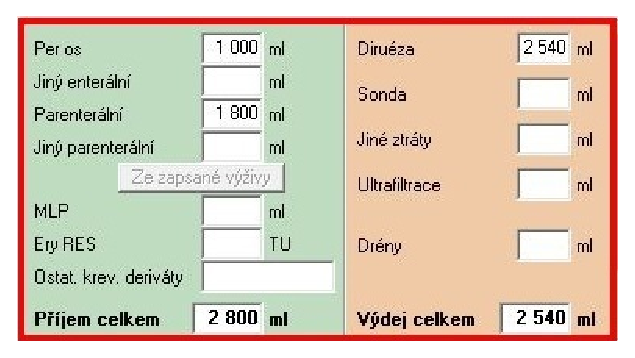
\includegraphics{img/medicalc/WM_bilance_tekutin.eps}
	\caption{Bilance tekutin (WinMedicalc)}
  \label{fig:WM_bilance_tekutin}
\end{figure}


Příjem a výdej tekutin se odečítají zdravotní sestry během dne několikrát, ke každé tekutině tedy během dne bude několik hodnot. Všechny hodnoty se ukládají do databáze, aby bylo možné sledovat jejich vývoj.

Zdravotní sestry zaznamenávají příjem a výdej tekutin na papír. Na konci dne přepíší údaje do WinMedicalcu.

\subsection{Invazivní přístupy}

Každý pacient může mít zaveden libovolný počet různých invazivních přístupů. Jedná se o katetry nebo drény. Každý invazivní přístup má vlastní specifikaci (číslo, název, umístění, hloubku zavedení, datum zavedení a počet dnů zavedení). Určité invazivní přístupy lze nechat v pacientovi zavedeny pouze po určitý počet dní (dle lékářských předpisů). Poté se musí vyměnit za nové nebo odebrat. Proto lze každý invazivní přístup v aplikaci označit požadavkem na výměnu. Následně jej lékař buď vymění, ve WinMedicalcu aktualizuje datum zavedení na datum výměny, nebo odebere a smaže ho ze seznamu invazivních přístupů. Změny invazivních přístupů do WinMedicalcu většinou zadává zdravotní sestra. Rozložení karty invazivní přístupů je na obrázku \ref{fig:WM_invazivni_pristupy}.

\begin{figure}[H]
	\centering
	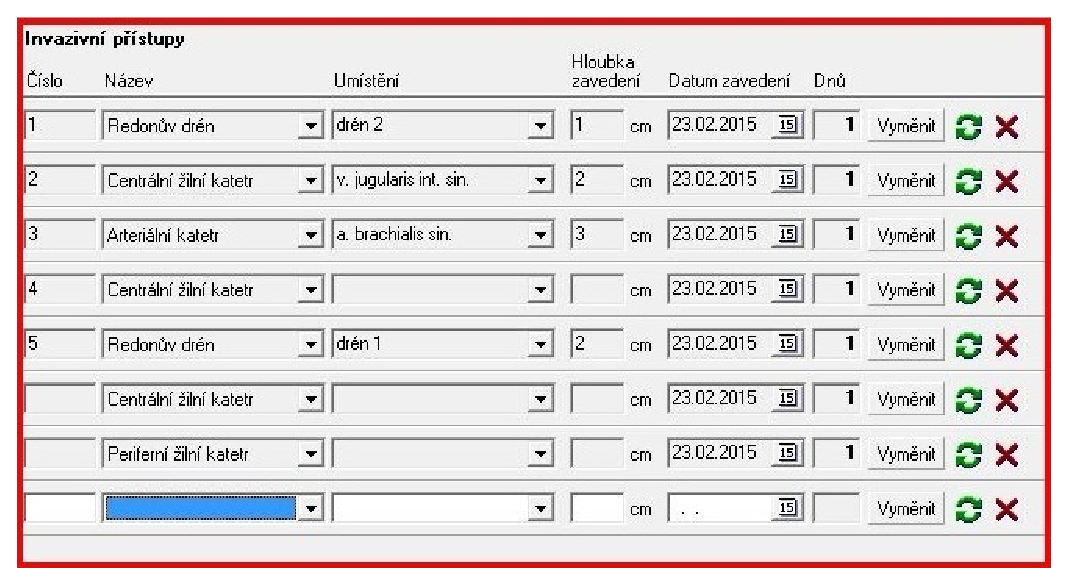
\includegraphics[width=1\textwidth]{img/medicalc/WM_invazivni_pristupy.eps}
	\caption{Invazivní přístupy (WinMedicalc)}
  \label{fig:WM_invazivni_pristupy}
\end{figure}


\subsection{Databáze}

Ve FN Plzeň je rozsáhlá databáze od Oraclu. V ní se ukládají prakticky všechny záznamy, včetně záznamů o pracovnících FN Plzeň, záznamů o pacientech a klinických událostech. Tato data se využijí ve vyvíjené aplikaci.

Jelikož přístup do databáze je pouze ve FN Plzeň, byla její část zkopírována do nového tablespace v Oracle databázi na ZČU. Tu jsme naplnili fiktivními testovacími daty, které odpovídají realným datům.
\chapter{Specifikace požadavků}
\label{ch:specifikace}

\section{Funkce aplikace}

Aplikace má pět částí:
\parskip=0em
\begin{itemize}
	\item Medikační karta
	\item Denní bilance tekutin
	\item Hodinová bilance tekutin
	\item Invazivní přístupy
	\item Fyziologie
\end{itemize}
\parskip=1em

Medikační karta nahrazuje tištěnou medikační kartu. Její vzhled odpovídá tištěné formě (tabulka se seznamem léků a jednotlivýma hodinama). Podání ordinovaného léku se bude moci provést DoubleClickem, nebo se jednoduchým kliknutím zobrazí dialog, ve kterém může uživatel editovat jednotlivé ordinace daného léku.

Denní bilance tekutin odpovídá bilanci tekutin ve WinMedicalc. Umožňuje zadávat množství příjmu a výdeje tekutin (celkovou hodnotu nebo nově naměřenou hodnotu)

Hodinová bilance tekutin je podobná denní bilanci tekutin. Ukazuje příjem a výdej tekutin v danou hodinu. Dále umožňuje zobrazit příjem a výdej tekutin ve všech hodinách.

Záložka invazivních přístumů odpovídajá invazivním přístupům ve WinMedicalcu. Zobrazuje zavedené invazivní přístupy a jejich popis. Umožňuje přístupy editovat, označit požadavkem na výměnu, přidat a smazat.

Záložka fyziologie zobrazuje záznamy životních funkcí pacienta. Záznamy lze přidat, editovat, nebo smazat.


\section{Kontext systému}

Aplikace je kompatibilní s informačím systémem FN Plzeň. Doplňuje aplikaci WinMedicalc, systémová integrita mezi oběmi aplikacemi není. Data jsou uložena v Oracle databázi nemocnice.

S vyvíjenou aplikací budou pracovat výhradně zdravotní sestry. Použití aplikace MediTab a WinMedicalc znázorňuje kontextový diagram na obrázku \ref{fig:kontext}.

\begin{figure}[H]
	\centering
	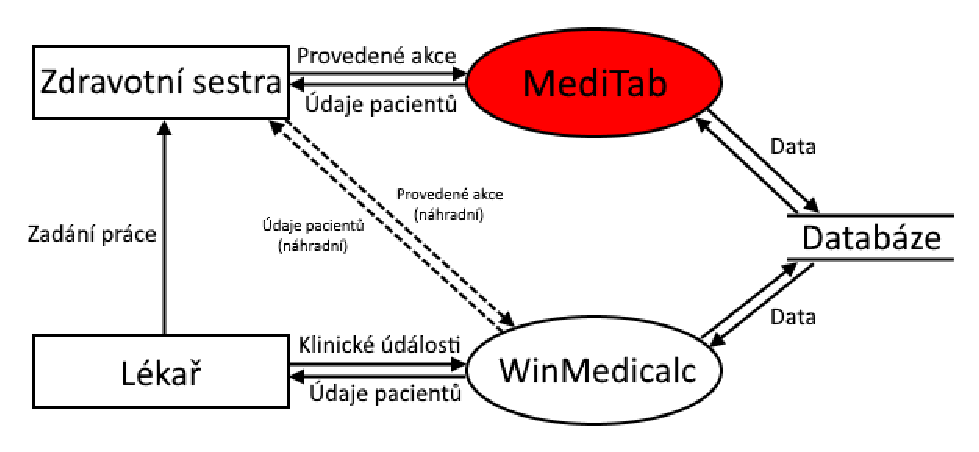
\includegraphics[width=0.8\textwidth]{img/kontext.eps}
	\caption{Kontextový diagram}
  \label{fig:kontext}
\end{figure}


\section{Technické parametry}

Aplikace běží na systému Microsoft Windows 8.1 64bit. Je vyvíjená na platformě Microsoft .NET Framework 4.5 v jazyce C\#.

Aplikace je kompatibilní s informačním systémem FN Plzeň a bude doplňovat program WinMedicalc. Systémová integrita mezi oběmi aplikacemi není, pouze jsou využity některé funkční prvky WinMedicalcu.

\subsection{Tablet}

SIS FN Plzeň vybralo HP ElitePad 1000G2 Healthcare Tablet, který je schválený pro použití v nemocničním prostředí. Tento tablet má antibakteriální povrchovou úpravu a odolnější konstrukci.

\noindent
Specifikace:

\noindent
\begin{tabular}{l l}
	Operační systém: & Microsoft Windows 8.1 64bit\\
	Procesor: & Intel Atom Z3795 (1.6 GHz, 2 MB cache, 4 jádra)\\
	Operační paměť: & 4 GB LPDDR3 SDRAM (1067 MHz)\\
	Interní paměť: & 128 GB eMMC\\
	Grafická karta: & Intel HD Graphics\\
	Displej: & 10.1" 1920 x 1200 (WUXGA)\\
	Výstupy: & 1 x USB 3.0, 1 x HDMI
\end{tabular}


\section{Databáze}

Přístup do databáze FN Plzeň je pouze ze zařízení, které jsou připojeny k doméně FN Plzeň. Proto byla část databáze potřebná pro vývoj aplikace zkopírována do nového tablespace v Oracle databázi na ZČU. Tabulky, ke kterým aplikace MediTab přistupuje jsou v ERA modelu na obrázku \ref{fig:era}. Kopie databáze je naplněna fiktivními testovacími daty, které odpovídají realným datům.

\begin{figure}[H]
	\centering
	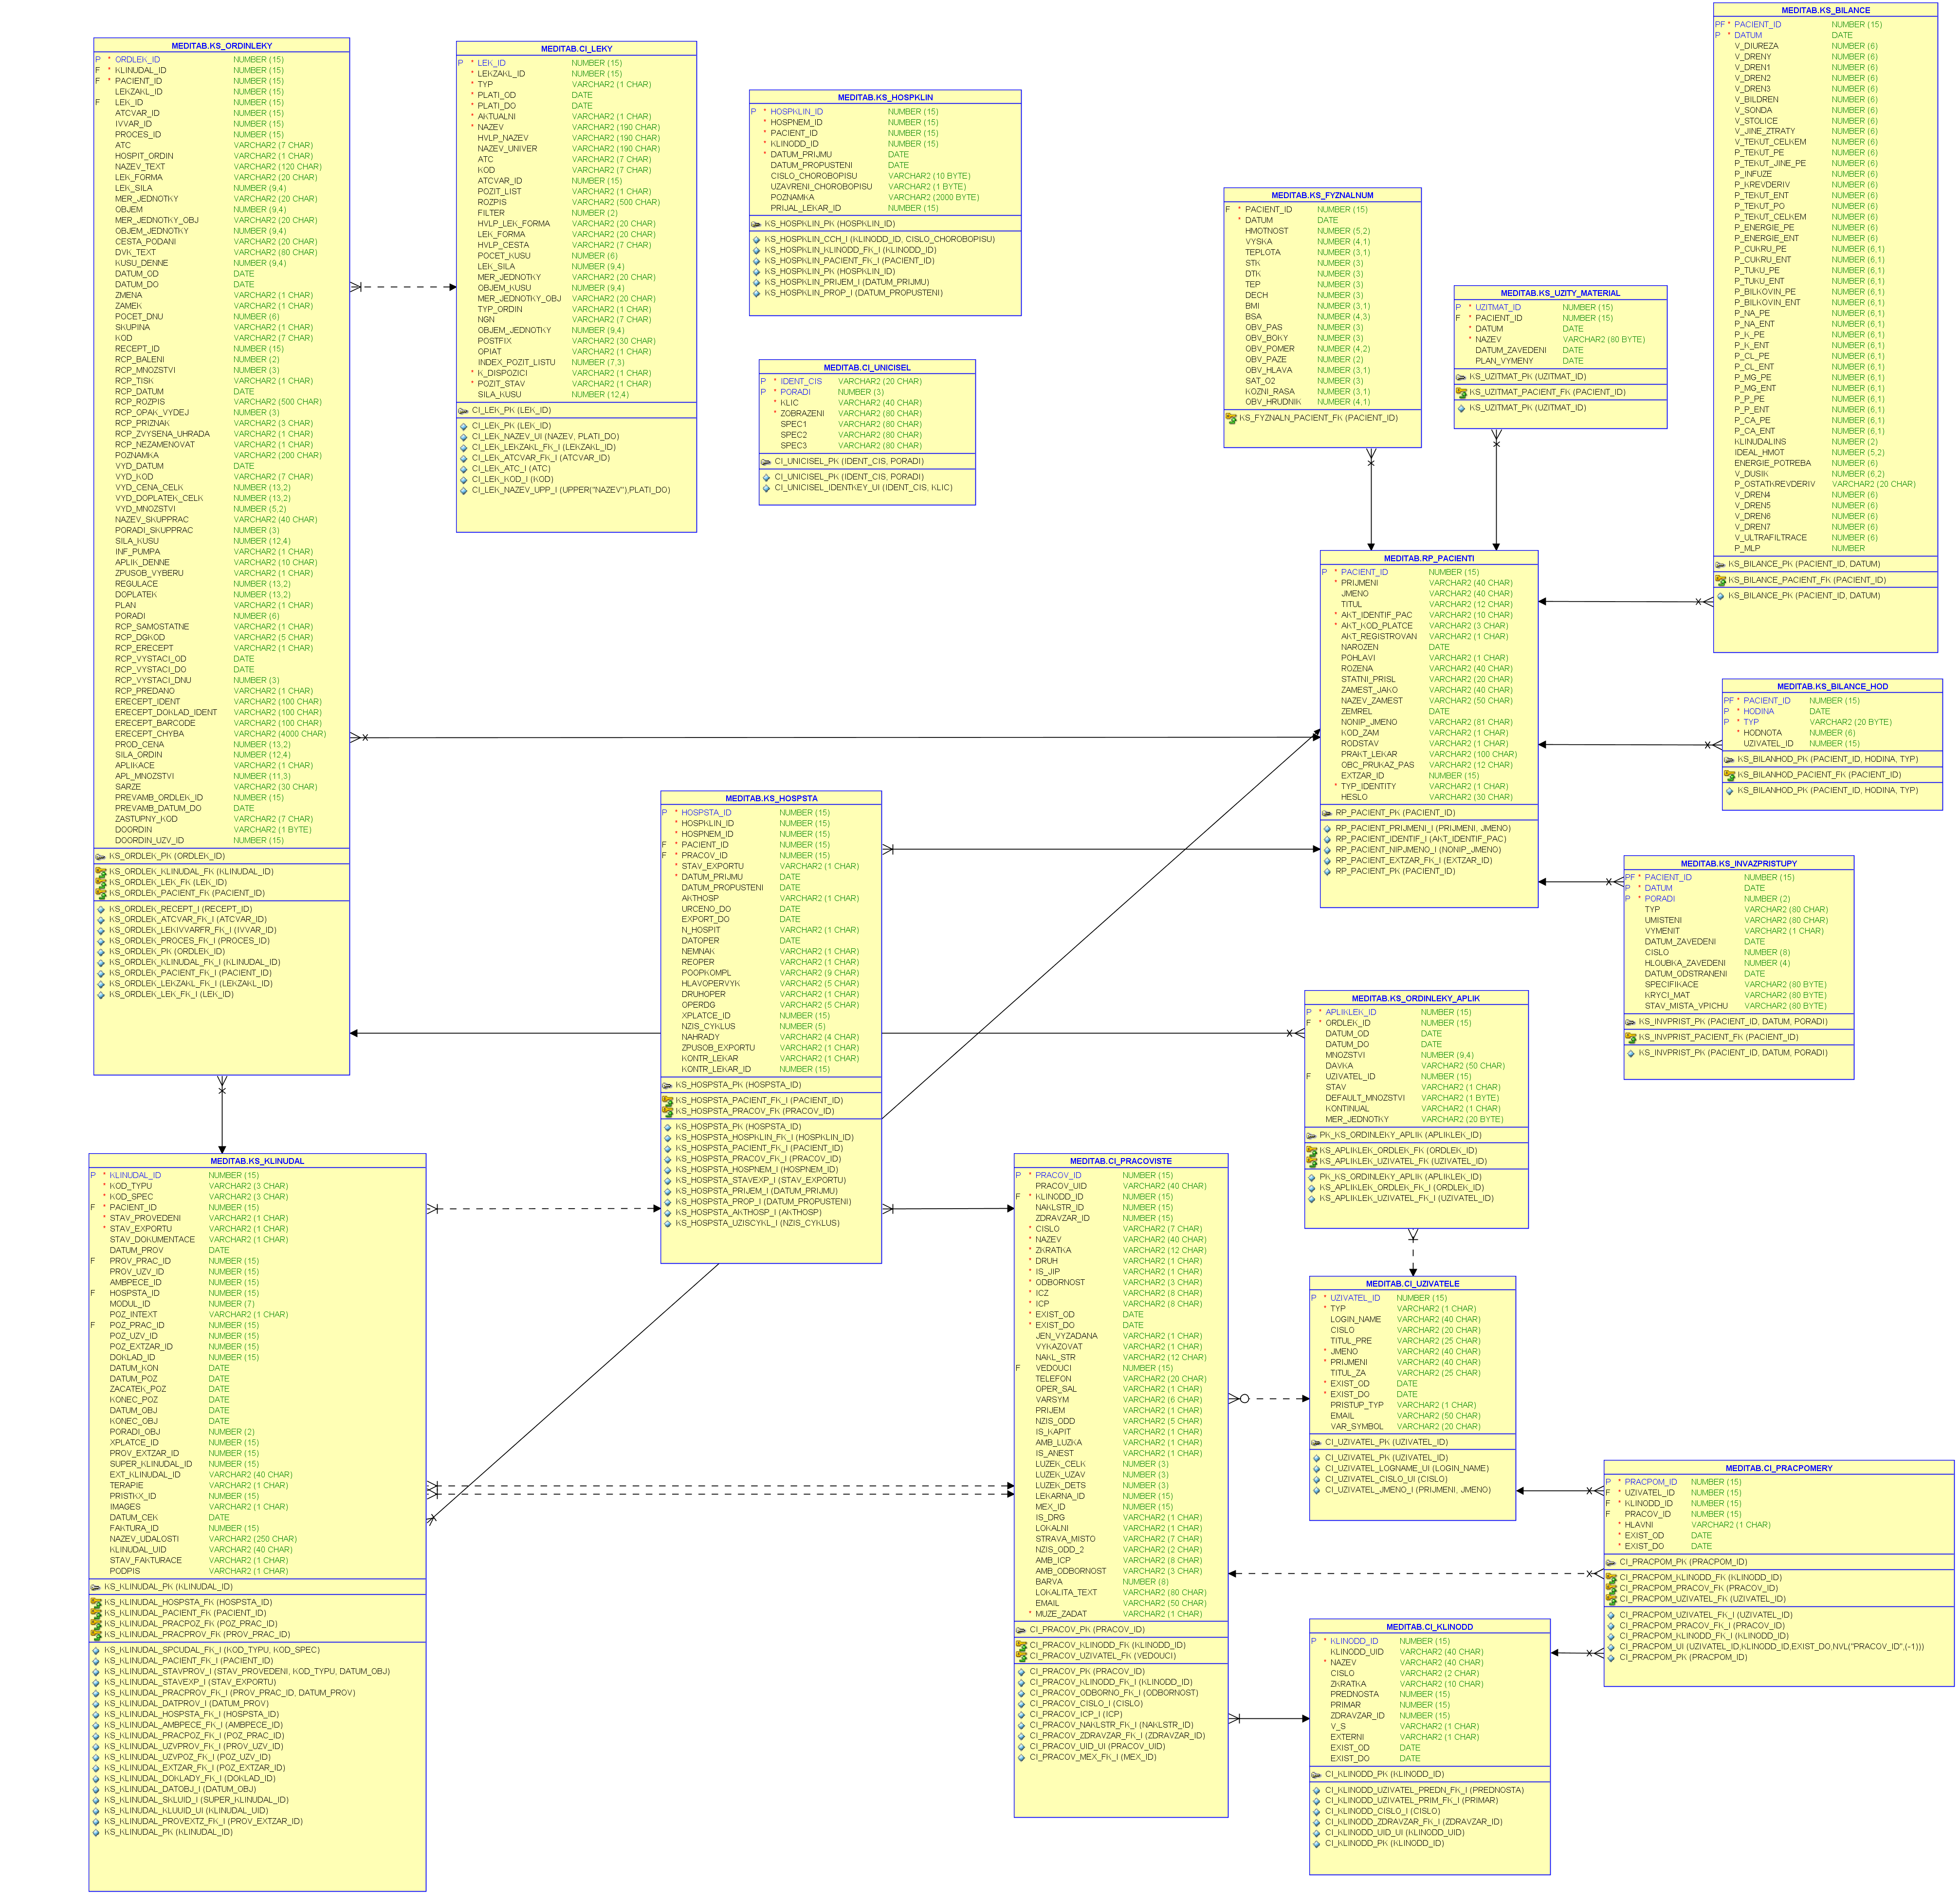
\includegraphics[width=1\textwidth]{img/ERA.eps}
	\caption{ERA model části databáze k vývoji aplikace}
  \label{fig:era}
\end{figure}

\setlength{\parskip}{1em}

\chapter{Návrh uživatelského rozhraní}

Pro usnadnění práce s aplikací je vhodné co nejvíce přizpůsobit vzhled aplikace vzhledu WinMedicalcu, na který jsou pracovníci FN Plzeň zvyklí. Proto jsem zvolil pro grafické uživatelské rozhraní knihovnu Windows Forms (System.Windows.Forms) místo novějšího WPF.

Grafické uživatelské rozhraní bude řešeno dynamicky pro možnost použití aplikace na jiných zařízeních.

Od vyvíjené aplikace je vyžadována vysoká spolehlivost. Proto musí být pečlivě otestováná přímo v prostředí FN Plzeň na nemocniční databázi a proveden testovací provoz. Na oddělení bude více tabletů pro případ, že by se některý rozbil či ztratil. Při selhání aplikace mohou sestry vždy použít program WinMedicalc nainstalovaný na počítači v sesterně, který je přímo připojen do interní sítě nemocnice. Výpadek databázového serveru nebo sítě řeší IT oddělení FN Plzeň.

\section{Přihlášení}

Jednoduchý dialog pro přihlášení uživatele do aplikace. Obsahuje textové pole pro jméno a pro heslo a dvě tlačítka pro potvrzení a zrušení přihlášení. Automaticky se zobrazí přes hlavní obrazovku při spuštění aplikace.

\section{Výběr pacientů}

Po přihlášení se zobrazí hlavní obrazovka aplikace. Na středu bude seznam pacientů na daném oddělení nebo lůžku (dle výběru z databáze). U každého pacienta bude zobrazeno jeho ID, příjmení, jméno a identifikační číslo (většinou rodné číslo).

V horní části obrazovky bude menu s možností odhlášení uživatele a zobrazení nápovědy. V dolní části statusbar s informacemi o přihlášeném uživateli a verzí aplikace. Vpravo bude tlačítko pro ukončení aplikace.

\section{Karta pacienta}

Po výběru pacienta se zobrazí obrazovka s jednotlivými kartami pacienta. Karty jsou Medikace, Denní bilance tekutin, Hodinová bilance tekutin a Invazivní přístupy. K dispozici bude vždy jen jedna varianta bilance tekutin dle oddělení, na kterém se tablet nachází (bude určeno v nastavení aplikace).

V dolní části obrazovky bude statusbar s informacemi o přihlášeném uživateli, vybraném pacientovi a verzí aplikace. Vpravo pak tlačítko pro návrat k výběru pacientů a tlačítko oprav.

\subsection{Ordinované léky}

Karta ordinovaných léků bude podobná tištěné medikační kartě. Jedná se o tabulku s názvem léku, předepsaným dávkováním a jednotlivými hodinami dávkování. V tabulce bude vyznačeno předepsané podání léku šedě a provedené podání léku zeleně s množstvím pro danou hodinu.

\subsection{Denní bilance tekutin}

Denní bilance tekutin bude rozdělena na dvě části pro příjem a výdej tekutin stejně jako tomu je ve WinMedicalcu. Příjem tekutin bude podbarven zeleně, bude obsahovat 7 položek, celkový součet a tlačítko pro uložení dat. Výdej tekutin bude podbarven červeně, bude obsahovat 5 položek, celkový součet a tlačítko pro uložení dat. U každé položky bude textové pole pro zadání nové celkové hodnoty a textové pole pro zadání nové hodnoty, která se přičte k původní.

\subsection{Hodinová bilance tekutin}

Hodinová bilance bude rozložením podobná denní bilanci tekutin. Pouze místo dvou textových polí bude mít jen jedno pro zadání hodnoty v aktuální hodinu. Dále tam bude u každé tekutiny tlačítko pro zobrazení seznamu příjmu nebo výdeje tekutiny v jednotlivých hodinách. Do tohoto seznamu se bude moci zapisovat pouze v určitých hodinách dle oddělení.

Tato karta není ve WinMedicalcu.

\subsection{Invazivní přístupy}

Karta invazivních přístupů bude mít podobný vzhled jako ve WinMedicalcu. Každý invazivní přístup bude obsahovat číslo, název, umístění, hloubku zavedení, datum zavedení, počet dnů zavedení, specifikaci, materiál katetru či drénu, stav místa zavedení a tři tlačítka - požadavek na výměnu, výměna a zrušení invazivního přístupu.

Jako poslední položka bude možnost přidání nového invazivního přístupu. Název, umístění a meteriál se bude vybírat ze seznamu. Datum bude nastaven na aktuální datum a počet dnů na 1. Číslo a hloubka zavedení bude číselná hodnota, specifikace a stav bude volně vypisovatelné. Tato položka bude mít pouze jedno tlačítko pro přidání.

\section{Opravy}

Po stisknutí tlačítka oprav se zobrazí seznam možných oprav provedených úkonů (ty budou časově omezeny dle oddělení). Každá položka bude obsahovat číslo opravy, datum a čas provedení úkonu, informace o provedeném úkonu a tlačítko pro vrácení úkonu. V dolní části bude tlačítko pro zavření seznamu.
\chapter{Implementace}

Grafické uživatelské rozhraní je implementováno knihovnou System.Windows.Forms. Aplikace by měla fungovat rychle, proto je priorita procesu nastavena na RealTime. Tak je zajišteno, že plánovač procesoru upřednostní aplikaci před aplikacemi s nižší prioritou.

Aplikace musí být odolná proti neplatným vstupům. Veškeré zapisované hodnoty se musí kontrolovat na správný formát a rozsah. Proto není možné zapisovat do jednotlivých komponent pomocí systémové klávesnice, ale pouze klávesnicí aplikace (viz kapitola \ref{ch:dialogy}). Další kontrola je v logické vrstvě aplikace.

V aplikaci jsou dvě hlavní okna, jedno pro výběr pacienta a druhé detail vybraného pacienta s jednotlivými záložkami. Okna s další funkčností jsou zobrazována jako dialogy.

Po spuštění aplikace se zobrazí okno výběru pacientů s prázdným seznamem pacientů a dialog pro přihlášení. Pro práci s aplikací musí být uživatel přihlášen a mít pracovní poměr na pracovišti, na kterém se tablet nachází.


\section{Přihlášení}

Pro přihlášení slouží jednoduchý dialog s dvěma TextBoxy, pro zadání uživatelského jména a hesla, a dvěma Buttony pro přihlášení a zrušení přihlášení. Uživatelské jméno ve FN Plzeň je vždy uppercase, proto jsou znaky v TextBoxu pro uživatelské jméno také uppercase. Znaky hesla jsou skryty symbolem *. Při úspěšném přihlášení se načtou údaje o uživateli a seznam pacientů na lůžkovém oddělení. Při neúspěšném přihlášení se zobrazí chybová hláška a údaje z TextBoxů se vymažou.

Přihlašovací dialog je na obrázku \ref{fig:login}.

\begin{figure}[H]
	\centering
	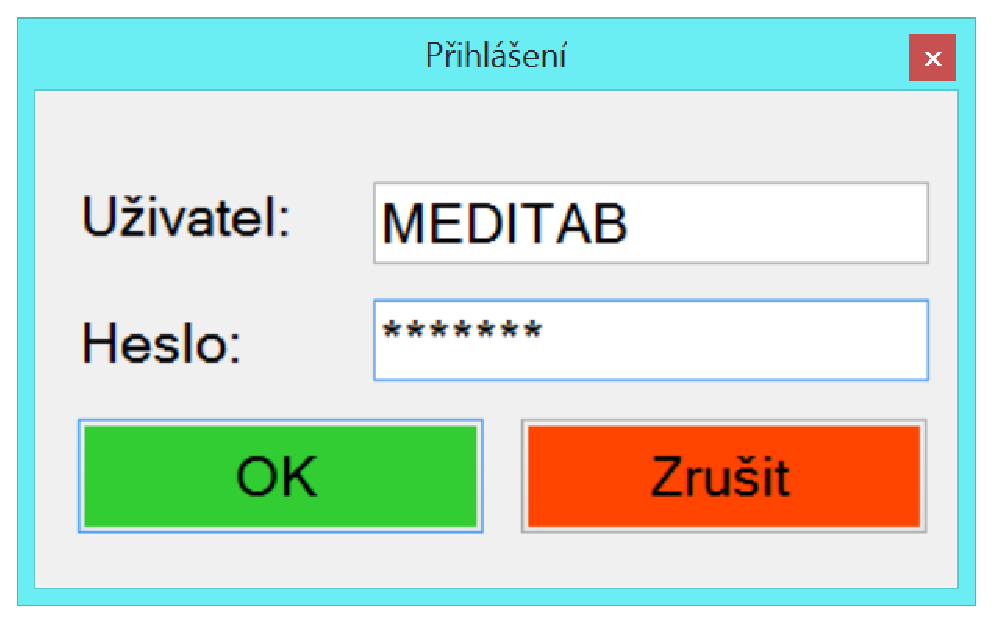
\includegraphics[width=0.4\textwidth]{img/meditab/login.eps}
	\caption{Přihlašovací dialog (MediTab)}
  \label{fig:login}
\end{figure}


\section{Výběr pacienta}

Po úspěšném přihlášení se zobrazí obrazovka se seznamem pacientů (viz obrázek \ref{fig:main}). Seznam pacientů je kolekce v ListView.

V horní části je MenuStrip obsahující dvě položky. První je tlačítko pro odhlášení, které odhlásí aktuálního uživatele a zobrazí dialog pro přihlášení, druhé tlačítko zobrazí nápovědu k aplikaci. Dole se nachází StatusStrip s informací o přihlášeném uživateli a verzí aplikace. Vravo je Button pro ukončení aplikace.

\begin{figure}[H]
	\centering
	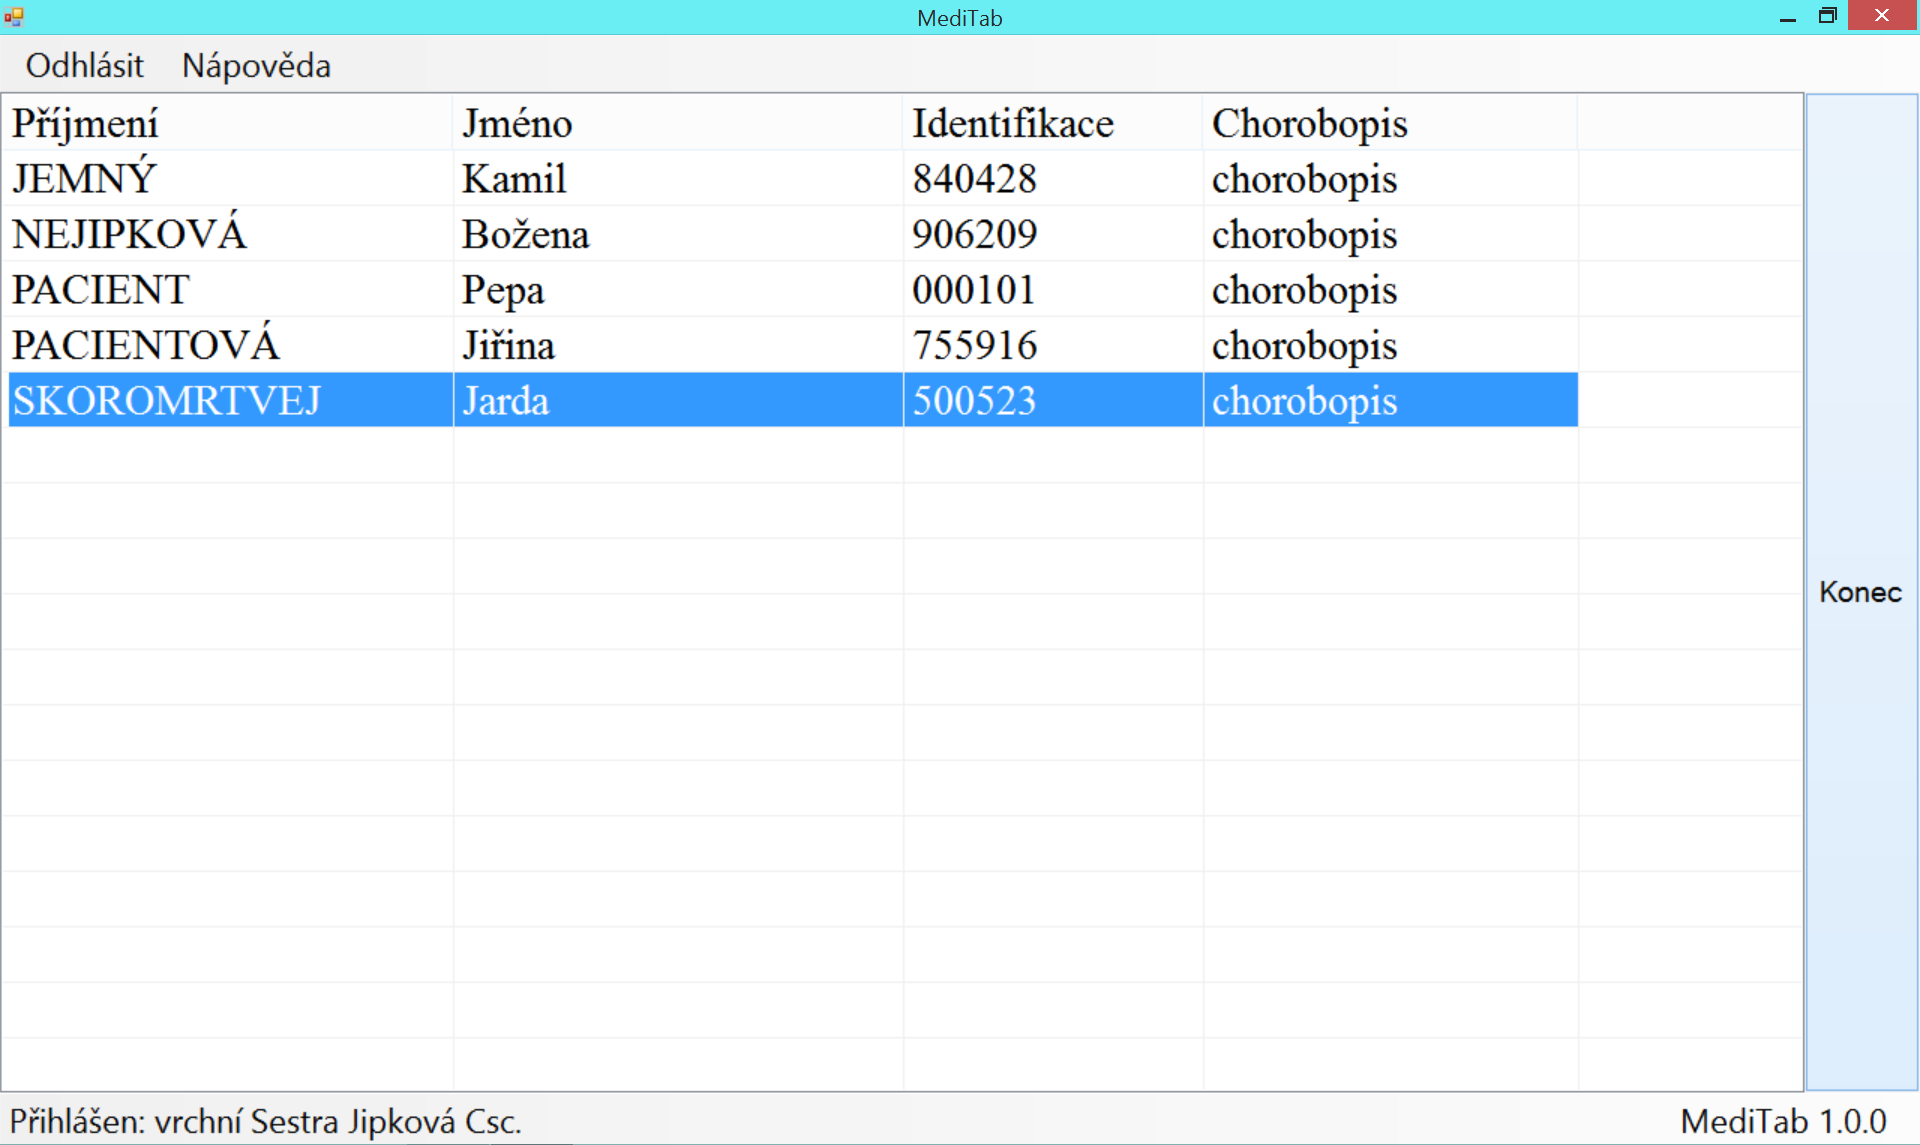
\includegraphics[width=1\textwidth]{img/meditab/main.eps}
	\caption{Výběr pacienta (MediTab)}
  \label{fig:main}
\end{figure}


Vybráním pacienta kliknutím na řádek v ListView se začnou stahovat data o pacientovi z databáze, vytvářet a inicializovat jednotlivé záložky. Uživatele o stavu načítání informuje načítací okno (viz obrázek \ref{fig:load}).

\begin{figure}[H]
	\centering
	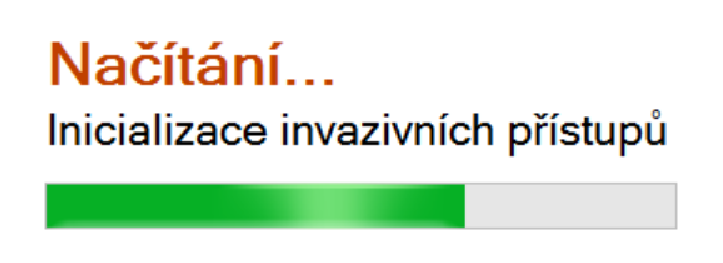
\includegraphics[width=0.4\textwidth]{img/meditab/loading.eps}
	\caption{Načítací okno (MediTab)}
  \label{fig:load}
\end{figure}



\section{Karta pacienta}

Hlavní částí okna je TabControl pro snadné přepínání mezi jednotlivými záložkami (TabPage). Vpravo je Button pro návrat k výběru pacientů a Button pro zobrazení oprav. Při otevřené záložce denní nebo hodinové bilance tekutin je zde Button pro návrat k výběru pacientů bez uložení hodnot. Vespod je StatusStrip s informací o přihlášeném uživateli, vybraném pacientovi a verzí aplikace.

\subsection{Ordinované léky}

Tabulku ordinovaných léků tvoří dva DataGridView (viz obrázek \ref{fig:medikace}). Oba DataGridView mají synchronizované vertikální scrollování. Scrollováním jednoho se nastaví veritikální scrollovací offset druhému.

\begin{figure}[H]
	\centering
	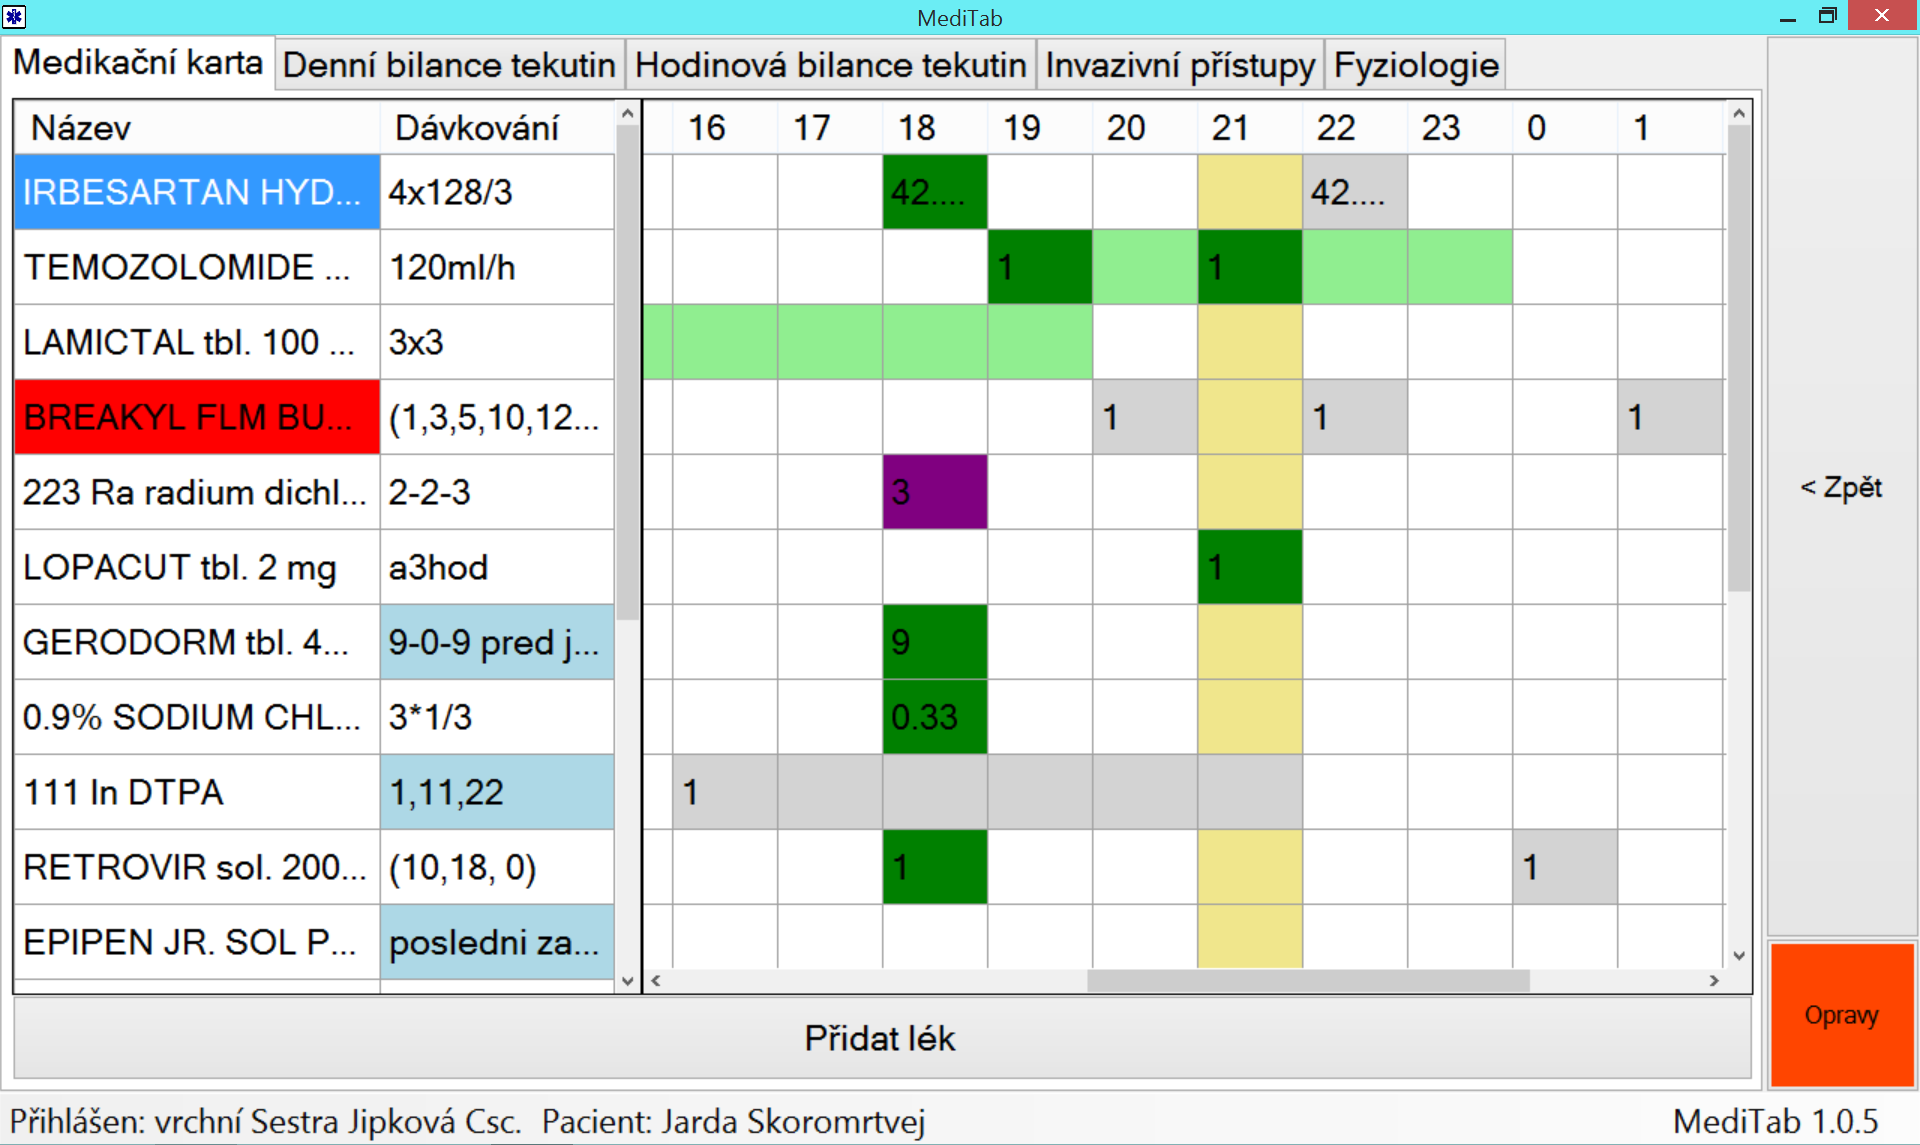
\includegraphics[width=1\textwidth]{img/meditab/medikace.eps}
	\caption{Ordinované léky (MediTab)}
  \label{fig:medikace}
\end{figure}

První DataGridView zobrazuje název léku a dávkování. Pokud je lék opiát, je políčko názvu léku podbarvebo červeně a pokud je u dávkování poznámka, políčko dávkování je podbarveno světle modře.

Druhý DataGridView zobrazuje tabulku jednotlivých ordinací. 24 sloupců představující jednotlivé hodiny je seřazeno od hodiny definované v konfiguraci jako počáteční hodina. Sloupec aktuální hodiny je podbarven khaki barvou vyjma řádek s ordinací v dané hodině. Ordinace má číselnou hodnotu dle množství, které má být/bylo podáno a je podbarvena:

\begin{itemize}
	\item Zeleně - provedená ordinace.
	\item Světle zeleně - provedená infuze (krom hodiny, kde infuze začíná, to je tmavě zelené). Infuze může mít definovaný konec, nebo je zobrazena do aktuální hodiny.
	\item Šedě - předepsané ordinace.
	\item Fialově - neprovedená ordinace.
\end{itemize}

Kliknutím na políčko DataGridView se zobrazí dialog podání ordinací (viz kapitola \ref{ch:ordinace} Podání ordinací) s vybranou ordinací (pokud existuje k dané hodině). Po zavření dialogu se aktualizuje celý řádek s lékem. Dvojitým kliknutím se rovnou provede podání ordinace v danou hodinu (podání pouze jednorázové ordinace, ne infuze).

Komponentě DataGridView nelze přiřadit událost Click a DoubleClick tak, aby se při dvojitém kliknutí nevyvolala událost jednoduchého kliknutí. Proto se při prvním kliknutí vytvoří vlákno, které na krátký čas pozastaví vykonání události jednoduchého kliknutí (zobrazení dialogu podání ordinací) a čeká se, jestli v této době uživatel klikne podruhé. Pokud ano, provede se jednorázové podání, pokud ne, zobrazí se dialog podání ordinací.

Vespod záložky je Button pro zobrazení dialogu přidání nového léku (viz kapitola \ref{ch:pridat_lek} Přidání nového léku).


\subsubsection{Podání ordinací}
\label{ch:ordinace}

Dialog podání ordinací rozložením kopíruje dialog ve WinMedicalc (viz obrázek \ref{fig:medikace}). Je rozdělen TableLayoutPanelem na šest části, tři řádky a dva sloupce.

\begin{figure}[H]
	\centering
	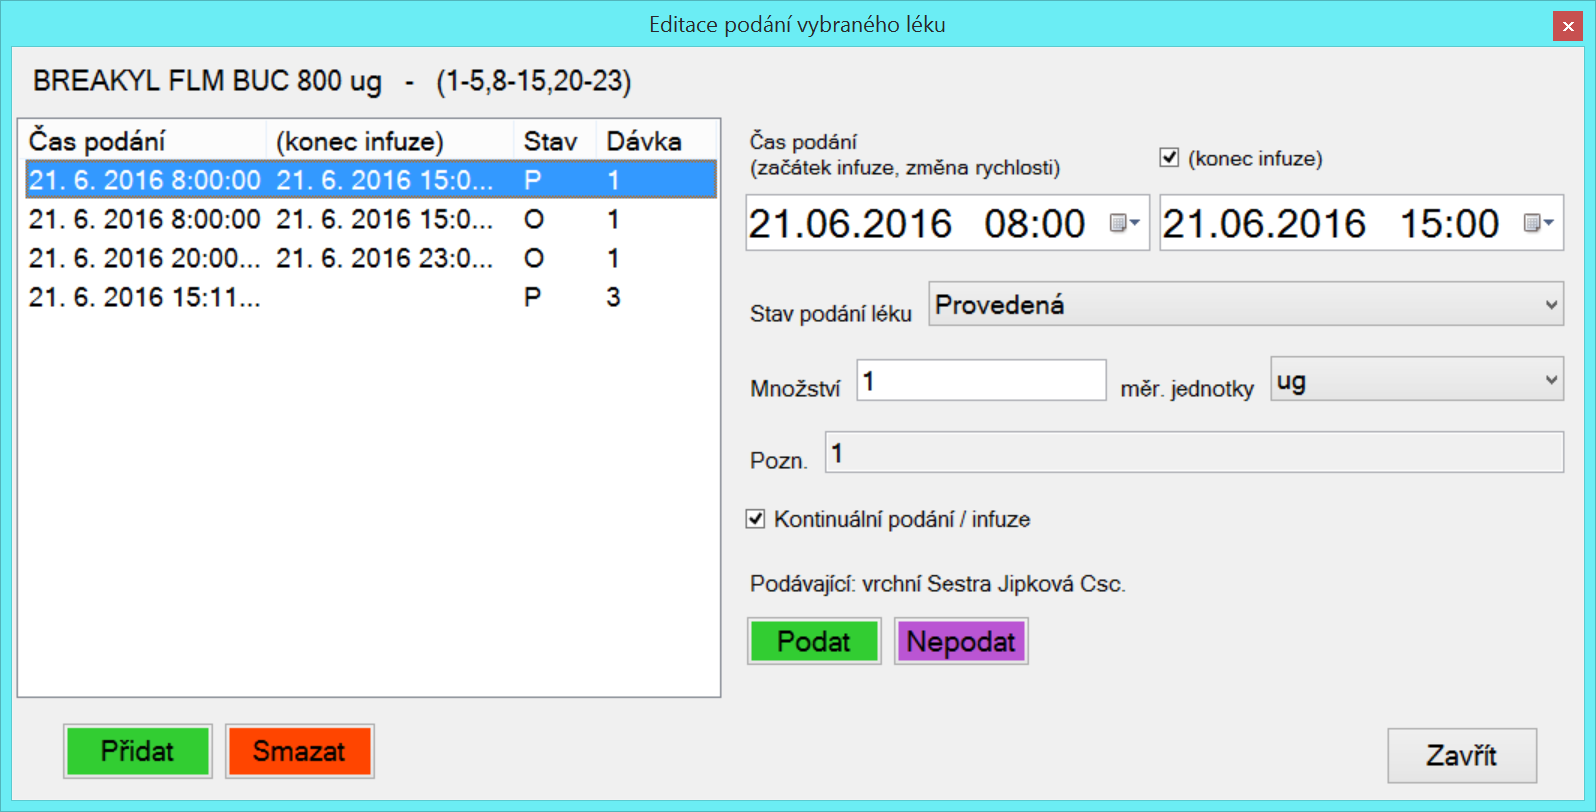
\includegraphics[width=0.8\textwidth]{img/meditab/ordinace.eps}
	\caption{Podání ordinací (MediTab)}
  \label{fig:ordinace}
\end{figure}

V prvním řádku je název léku a dávkování.

V druhém řádku prvním sloupci je seznam ordinací daného léku v ListView, v druhém sloupci pak detail vybrané ordinace. Vybráním ordinace ze seznamu (FocusedIndex) se zobrazí její detail. V případě, že se změní některá hodnota ordinace, se při výběru jiné nebo zavření dialogu současná uloží a případně se aktualizuje řádek v ListView.

Změna hodin v DateTimePickerech nastane přejetím prstu po komponentě (přímá změna hodnoty není na tabletu vhodná). V okamžiku vstupu do místa DateTimePickeru se uloží y-ová souřadnice, v okamžiku kdy se komponenta opustí, hodina se podle místa opuštění zvýší nebo sníží. Do poznámky lze zapisovat, pouze pokud je stav ordinace nastaven na nepodáno. Pokud ordinace nemá nastaveny vlastní jednotky, zobrazují se jednotky léku.

V posledním řádku jsou tlačítka na přidání nové ordinace, smazání ordinace a zavření dialogu. Button přidání ordinace vytvoří záznam v ListView ordinací, ordinace se uloží až při vybrání jiné ordinace nebo při zavření dialogu. Proto se při mazání ordinace zkontroluje, zda je daná ordinace v paměti. Pokud ano, odešle se požadavek na smazání, pokud ne, odstraní se pouze z ListView. Při zavření dialogu proběhne kontrola, zda právě zobrazená ordinace nebyla změněna, a případně se uloží.


\subsubsection{Přidání nového léku}
\label{ch:pridat_lek}

Dialog na obrázku \ref{fig:medikace_pridat_lek} umožní sestře přidat nový naordinovaný lék.

\begin{figure}[H]
	\centering
	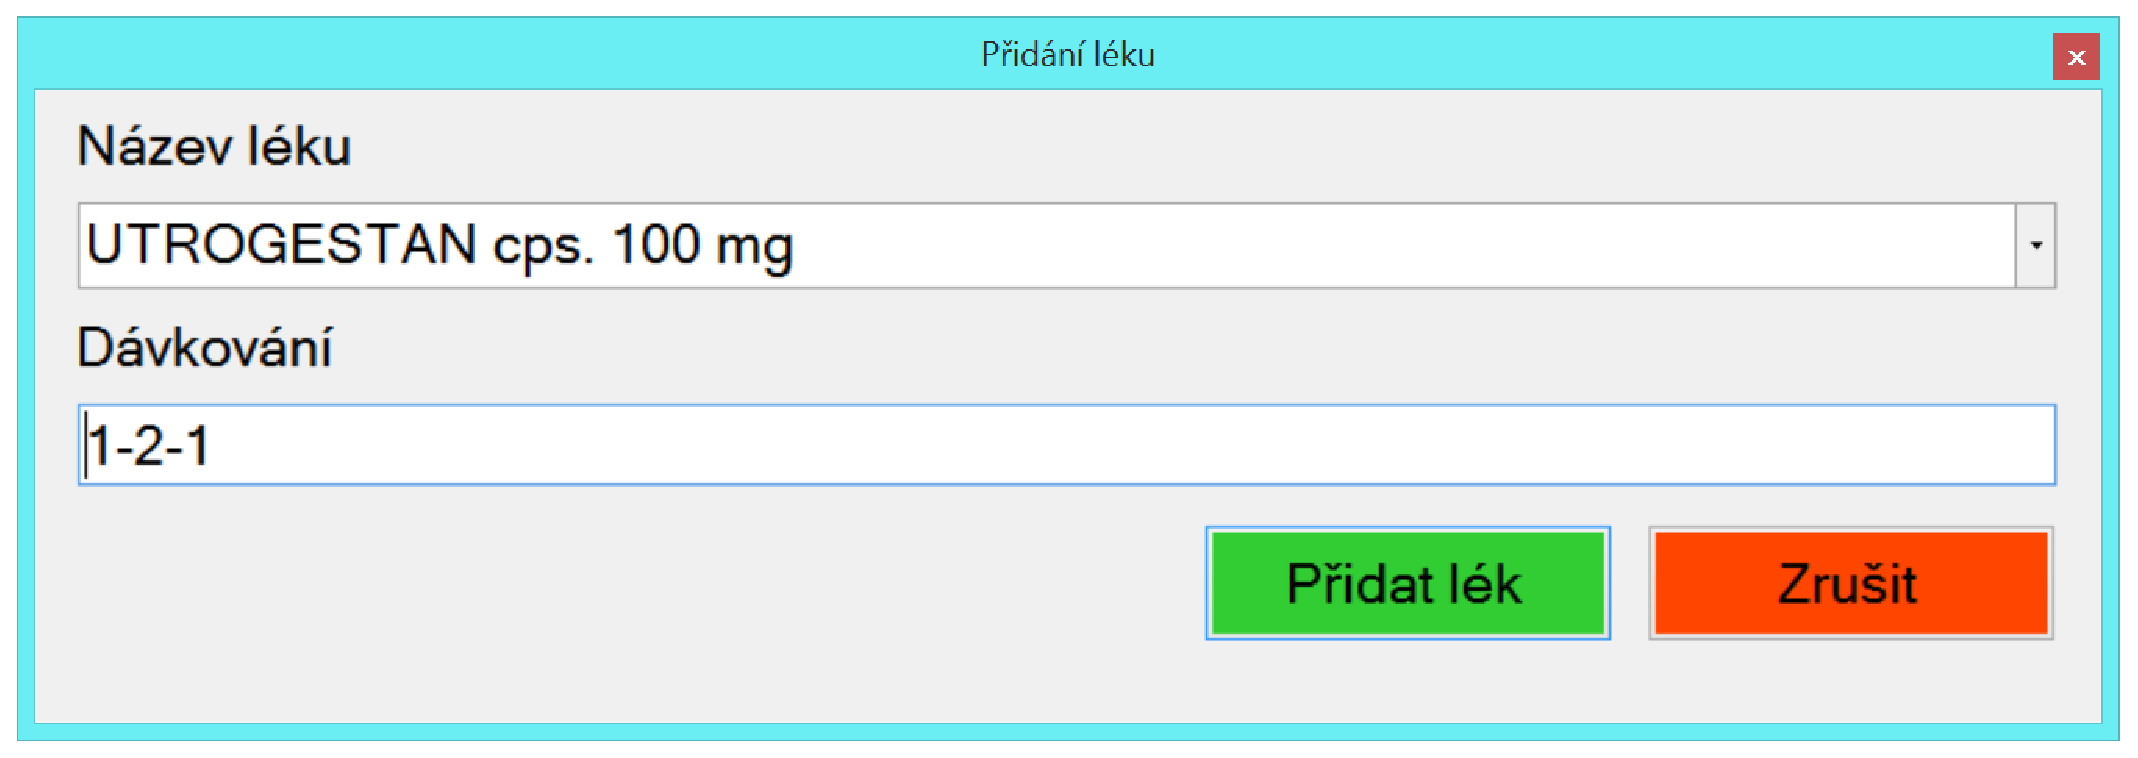
\includegraphics[width=0.6\textwidth]{img/meditab/medikace_pridat_lek.eps}
	\caption{Přidání nového léku (MediTab)}
  \label{fig:medikace_pridat_lek}
\end{figure}

V ComboBoxu se vybírá lék, který má být naordinován. Jelikož je léků velké množství a většina má více druhů balení, po napsání části názvu léku se v ComboBoxu zobrazí pouze léky obsahující tento text. V dávkování je uživatel motivován k zápisu podle standartů nemocnice, které mohou být rozparsovatelné a následně graficky znázorněné v medikační kartě. Pokud uživatel zadá podání nekorektně nebo vůbec, je o tom informován a předepsání léku s nekorektním dávkováním musí potvrdit.

Po zavření dialogu se nový lék přidá na poslední řádku v medikační kartě.


\subsection{Denní bilance tekutin}

Záložka denní bilance tekutin (na obrázku \ref{fig:bilance_den}) zobrazuje bilanci tekutin za celý den. Je rozdělena SplitContainerem na tekutiny příjmu (zelená) a tekutiny výdeje (červená). Každá tekutina má dva TextBoxy, první zobrazuje celkovou hodnotu za den (lze zadat novou hodnotu větší než původní), v druhém lze přičíst nově naměřenou hodnotu. Poslední hodnotou je celkový součet příjmu nebo výdeje všech tekutin.

Jednotlivé tekutiny jsou v paměti indexovány podle enumu \emph{Tekutiny}. Stejně tak jsou indexovány TextBoxy (TabIndex). Jelikož pole celkové hodnoty a pole pro zadání nově naměřené hodnoty jedné tekutiny náleží jednomu indexu v paměti (ale stále je nutné oba TextBoxy rozlišit), přičte se k indexu pole nové hodnoty konstanta 100 (při předávání hodnoty se odečte). Při ukládání hodnot se předává index TextBoxu a hodnota.

\begin{figure}[H]
	\centering
	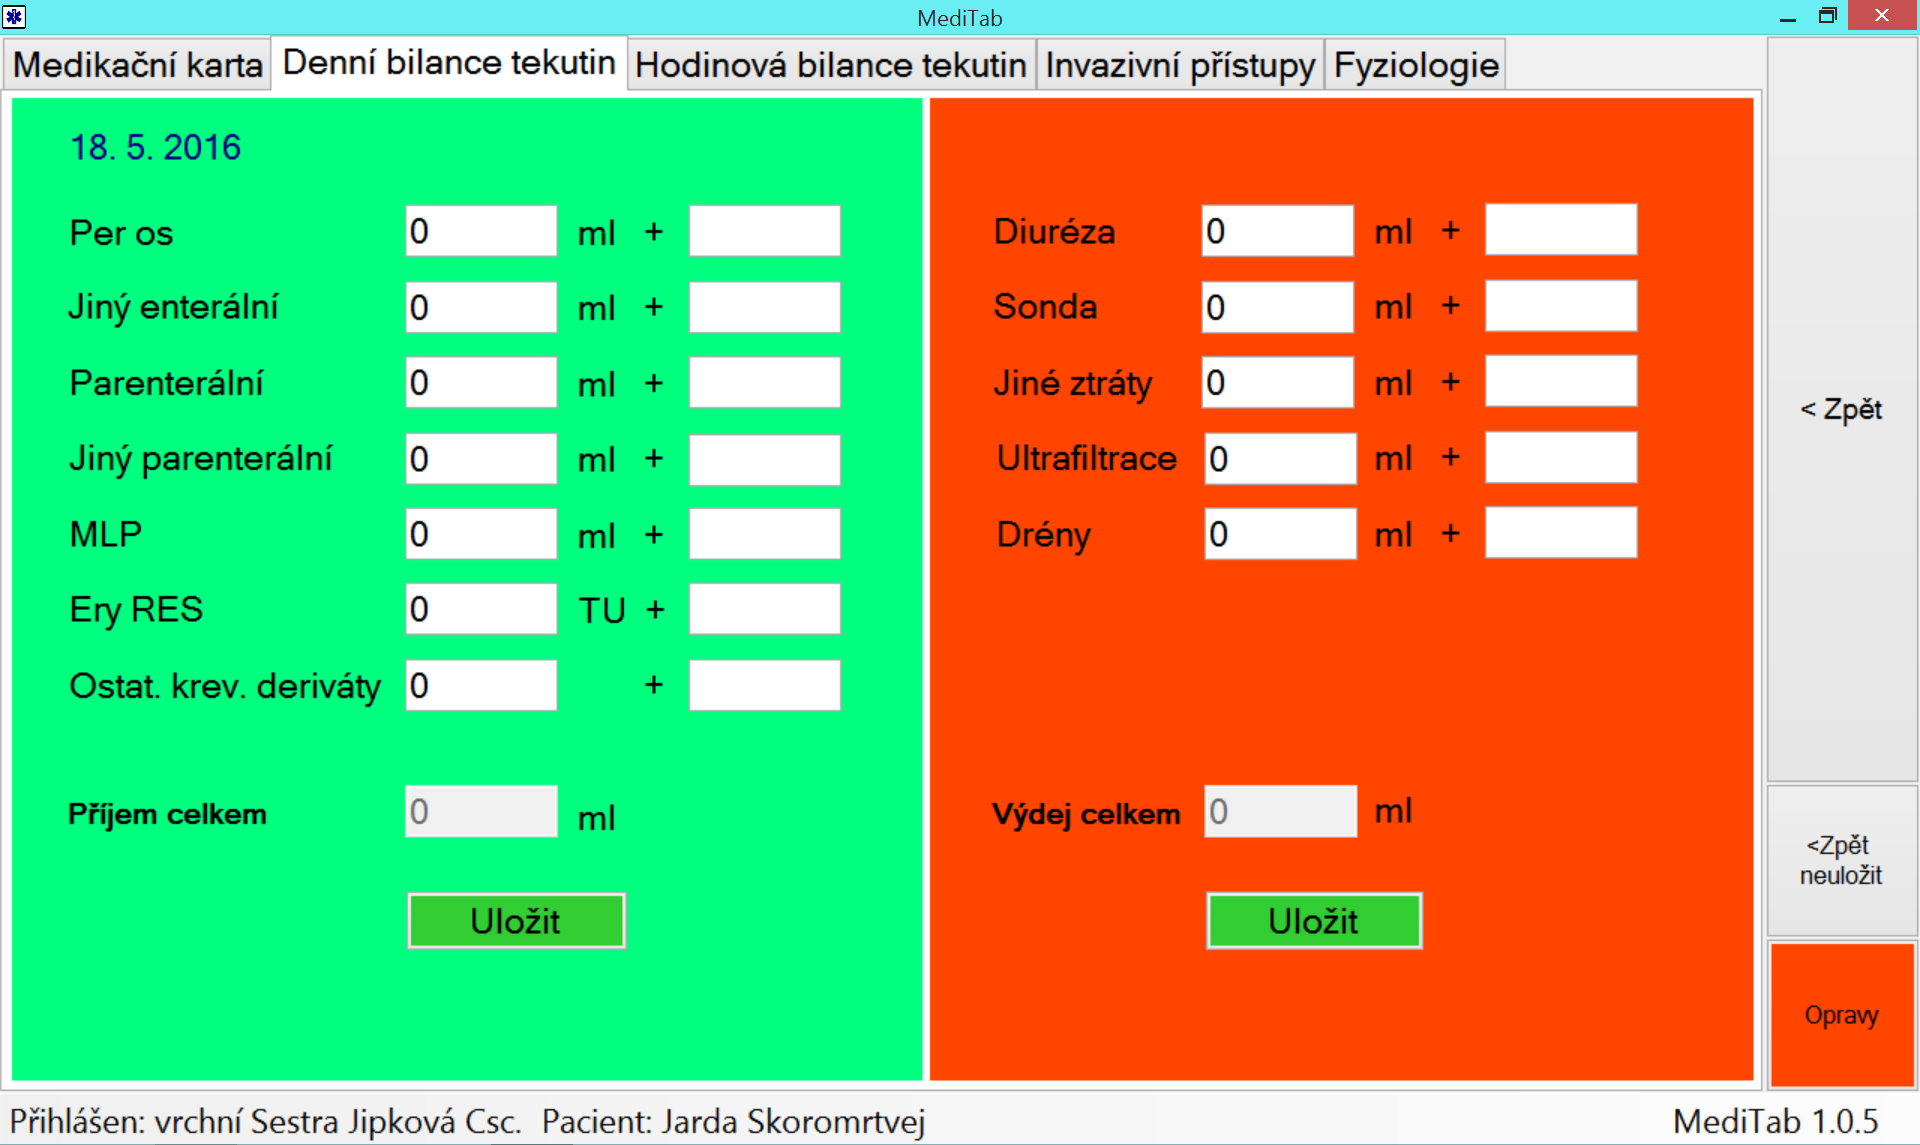
\includegraphics[width=1\textwidth]{img/meditab/bilance_den.eps}
	\caption{Denní bilance tekutin (MediTab)}
  \label{fig:bilance_den}
\end{figure}

Hodnoty se musí uložit kliknutím na Button \emph{Uložit}. Pokud uživatel přepne na jinou záložku, aplikace ho upozorní, že hodnoty neuložil, a zeptá se, jestli je chce uložit. Buttonem \emph{Zpět} se hodnoty uloží a vrátí se k výběru pacientů, Buttonem \emph{Zpět bez uložení} se vrátí k výběru pacientů bez uložení.

\subsection{Hodinová bilance tekutin}

Záložka hodinové bilance tekutin (na obrázku \ref{fig:bilance_hod}) zobrazuje bilanci tekutin za aktuální hodinu. Je rozdělena SplitContainerem na tekutiny příjmu (zelená) a tekutiny výdeje (červená). Každá tekutina má TextBox, který zobrazuje hodnotu v aktuální hodinu (lze zadat pouze jednu hodnotu v hodině) a Button, který zobrazí dialog se všemi hodinami k dané tekutině (viz obrázek \ref{fig:bilance_hod_detail}). Poslední dvě hodnoty jsou celkový součet příjmu nebo výdeje všech tekutin v dané hodině a za celý den.

Jednotlivé tekutiny jsou v paměti indexovány podle enumu \emph{Tekutiny}. Stejně tak jsou indexovány TextBoxy (TabIndex). Jelikož pole celkové hodnoty a pole pro zadání nově naměřené hodnoty jedné tekutiny náleží jednomu indexu v paměti (ale stále je nutné oba TextBoxy rozlišit), přičte se k indexu pole nové hodnoty konstanta 100 (při předávání hodnoty se odečte). Při ukládání hodnot se předává index TextBoxu hodnota a aktuální hodina.

\begin{figure}[H]
	\centering
	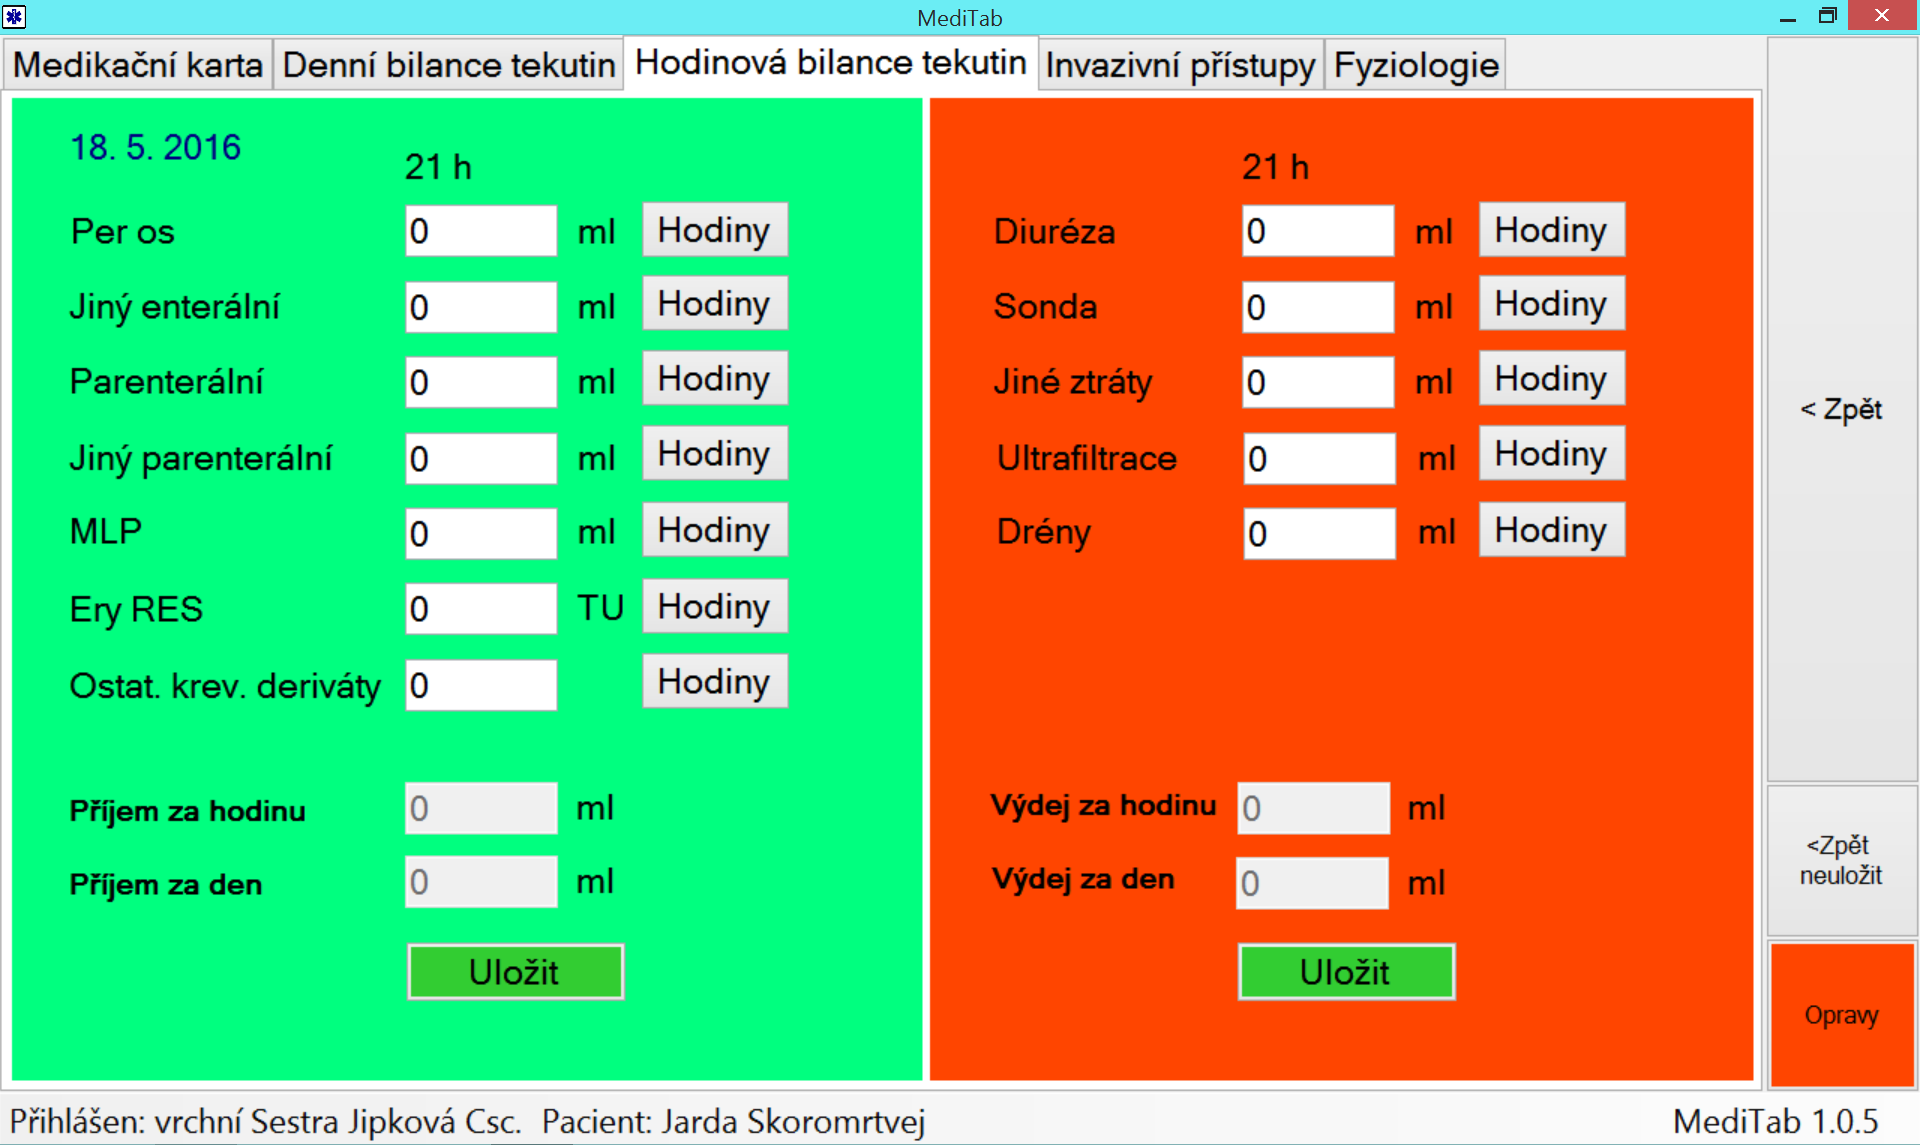
\includegraphics[width=1\textwidth]{img/meditab/bilance_hod.eps}
	\caption{Hodinová bilance tekutin (MediTab)}
  \label{fig:bilance_hod}
\end{figure}

Dialog s hodinovým detailem tekutiny obsahuje DataGridView s dvěma sloupci (hodina, hodnota). Vespod pak je součet všech hodinových hodnot dané tekutiny a tlačítko zavřít. Hodnoty k jednotlivým hodinám lze zadat kliknutím na dané políčko DataGridView. V hodinu lze zadat pouze jednu hodnotu.

\begin{figure}[H]
	\centering
	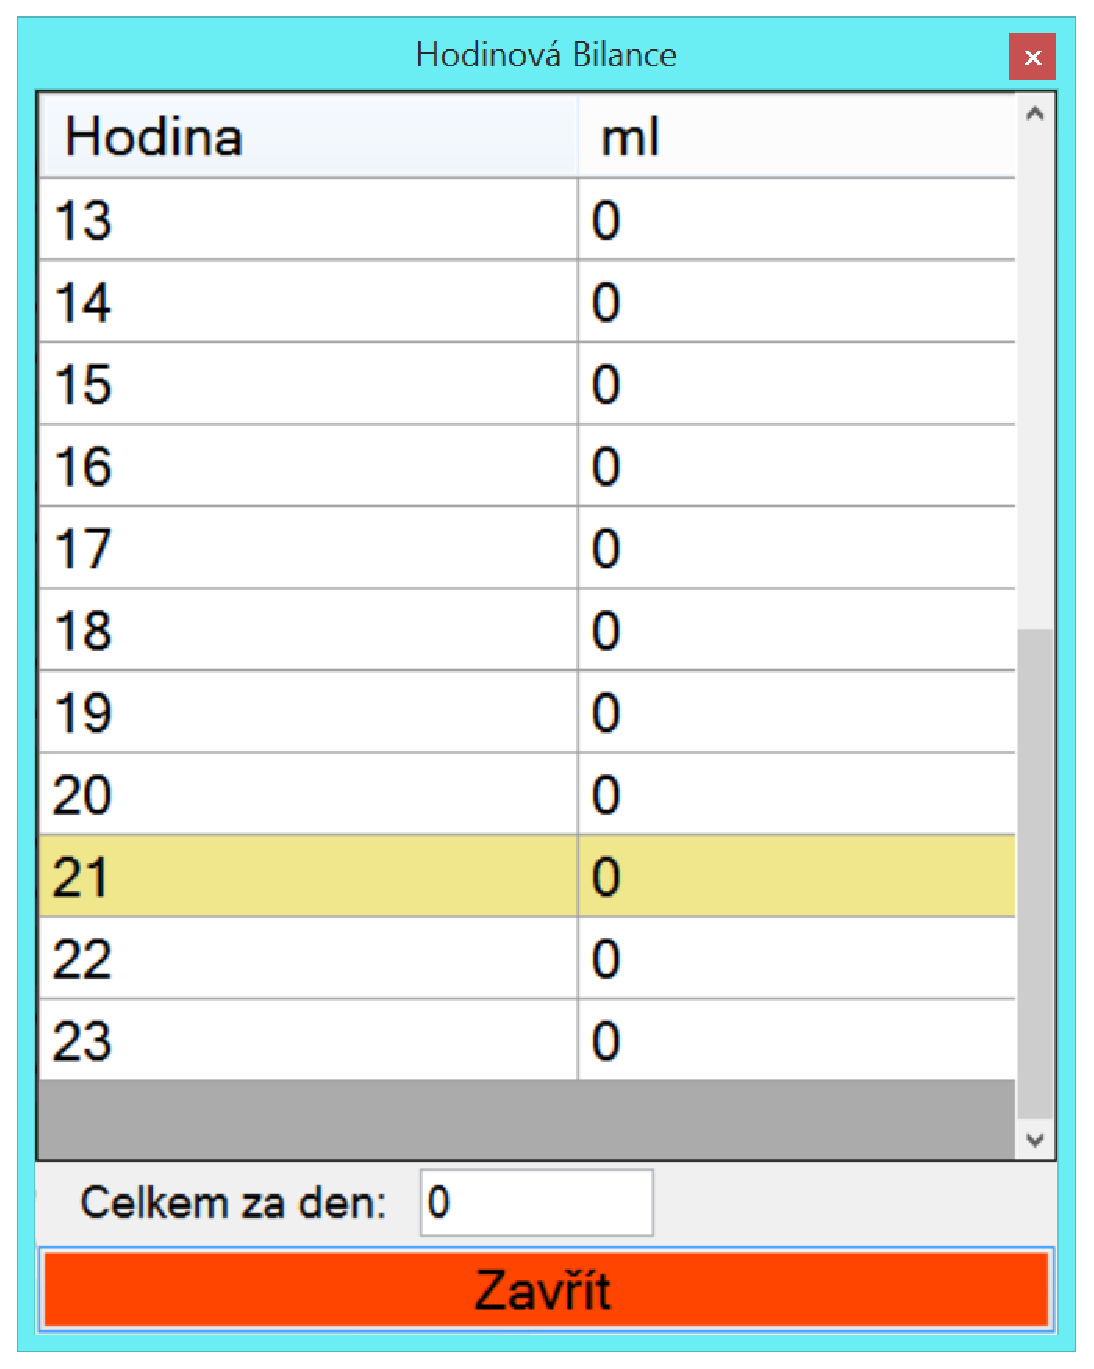
\includegraphics[width=0.3\textwidth]{img/meditab/bilance_hod_detail.eps}
	\caption{Hodinová bilance tekutin - hodinový detail tekutiny (MediTab)}
  \label{fig:bilance_hod_detail}
\end{figure}

Hodnoty se musí uložit kliknutím na Button \emph{Uložit}. Pokud uživatel přepne na jinou záložku, aplikace ho upozorní, že hodnoty neuložil, a zeptá se, jestli je chce uložit. Buttonem \emph{Zpět} se hodnoty uloží a vrátí se k výběru pacientů, Buttonem \emph{Zpět bez uložení} se vrátí k výběru pacientů bez uložení.


\subsection{Invazivní přístupy}
\label{ch:pristup}

V záložce invazivních přístupů (obrázek \ref{fig:invaz_pristup}) je každý invazivní přístup reprezentován vytvořenou komponentou PristupPanel, která dědí od FlowLayoutPanelu. V PristupPanelu jsou veškeré komponenty s informacemi o daném invazivním přístupu (ComboBoxy, TextBoxy, DateTimePicker) a ovládací tlačítka (Vyměnit, Aktualizuj, Vymaž). Panel je na střídačku podbarven ve dvou odstínech světle šedé pro lepší přehlednost.

První panel je pouze s Labely označujícími uspořádání komponent. Poslední panel umožňuje přidání nového invazivního přístupu. Tento panel má místo ovládacích tlačítek Button \emph{Přidat}. Přidáním nového invazivního přístupu se přístup uloží, místo Buttonu \emph{Přidat} zobrazí ovládací tlačítka a do záložky se přidá nový PristupPanel pro přidání dalšího přístupu.

\begin{figure}[H]
	\centering
	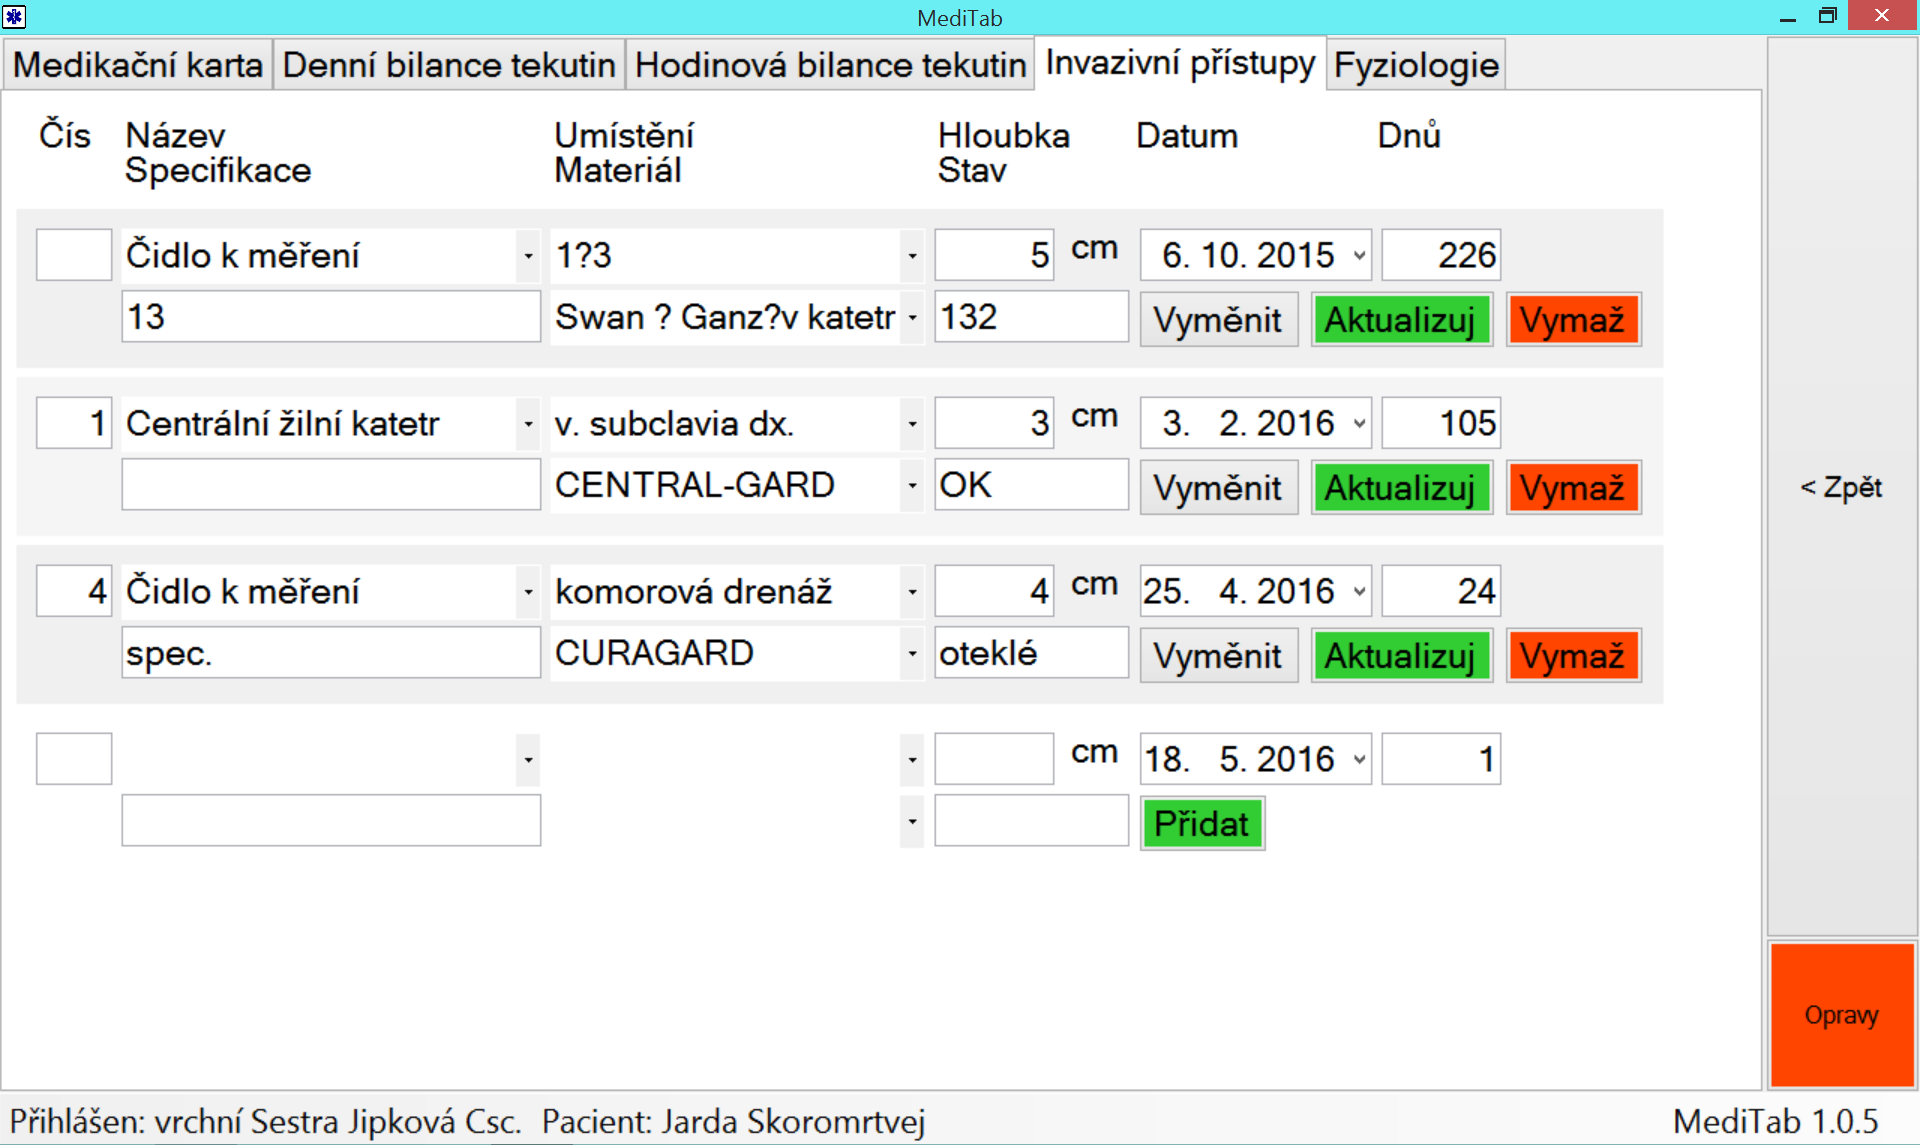
\includegraphics[width=1\textwidth]{img/meditab/invaz_pristup.eps}
	\caption{Invazivní přístupy (MediTab)}
  \label{fig:invaz_pristup}
\end{figure}

Scrollování tažením prstem na tabletu ve WinForms nereaguje správně. Vyvolá se scrollovací událost vrchní komponenty, ne kontejneru, ve kterém jsou komponenty umístěny. To jsem vyřešil vytvořením MessageFiltru \emph{MouseFilter} a \emph{TouchableLayoutPanelu}.

MouseFilter monitoruje systémové události, konkrétně stisk levého tlačítka myši (kliknutí prstem), uvolnění levého tlačítka myši a pohyb myši, a odešle je do jejich destinace (tj. komponenta, která se u MouseFilteru zaregistruje jako posluchač). 

TouchableFlowLayoutPanel dědí od FlowLayoutPanelu, a má tak stejné vlastnosti. Při jeho vytvoření zaregistruje reakce na scrollování (nastavení scrollovacího offsetu dle pohybu myši) událostem MouseFilteru. Stejně tak se musí zaregistrovat každý PristupPanel (nastavení scrollovacího offsetu rodičovského kontejneru).


\subsection{Fyziologie}

V záložce fyziologie (obrázek \ref{fig:fyziologie}) je každý záznam reprezentován vytvořenou komponentou FyziologiePanel, která dědí od FlowLayoutPanelu. Ve FyziologiePanelu je datum záznamu, TextBoxy s hodnotami životních funkcí pacienta a ovládací tlačítka (Upravit, Smazat).

První panel je pouze s Labely označujícími uspořádání komponent. Poslední panel umožňuje přidání nového záznamu. Tento panel má místo ovládacích tlačítek Button \emph{Přidat}. Přidáním nového záznamu se záznam uloží, místo Buttonu \emph{Přidat} zobrazí ovládací tlačítka a do záložky se přidá nový FyziologiePanel pro přidání dalšího záznamu.

\begin{figure}[H]
	\centering
	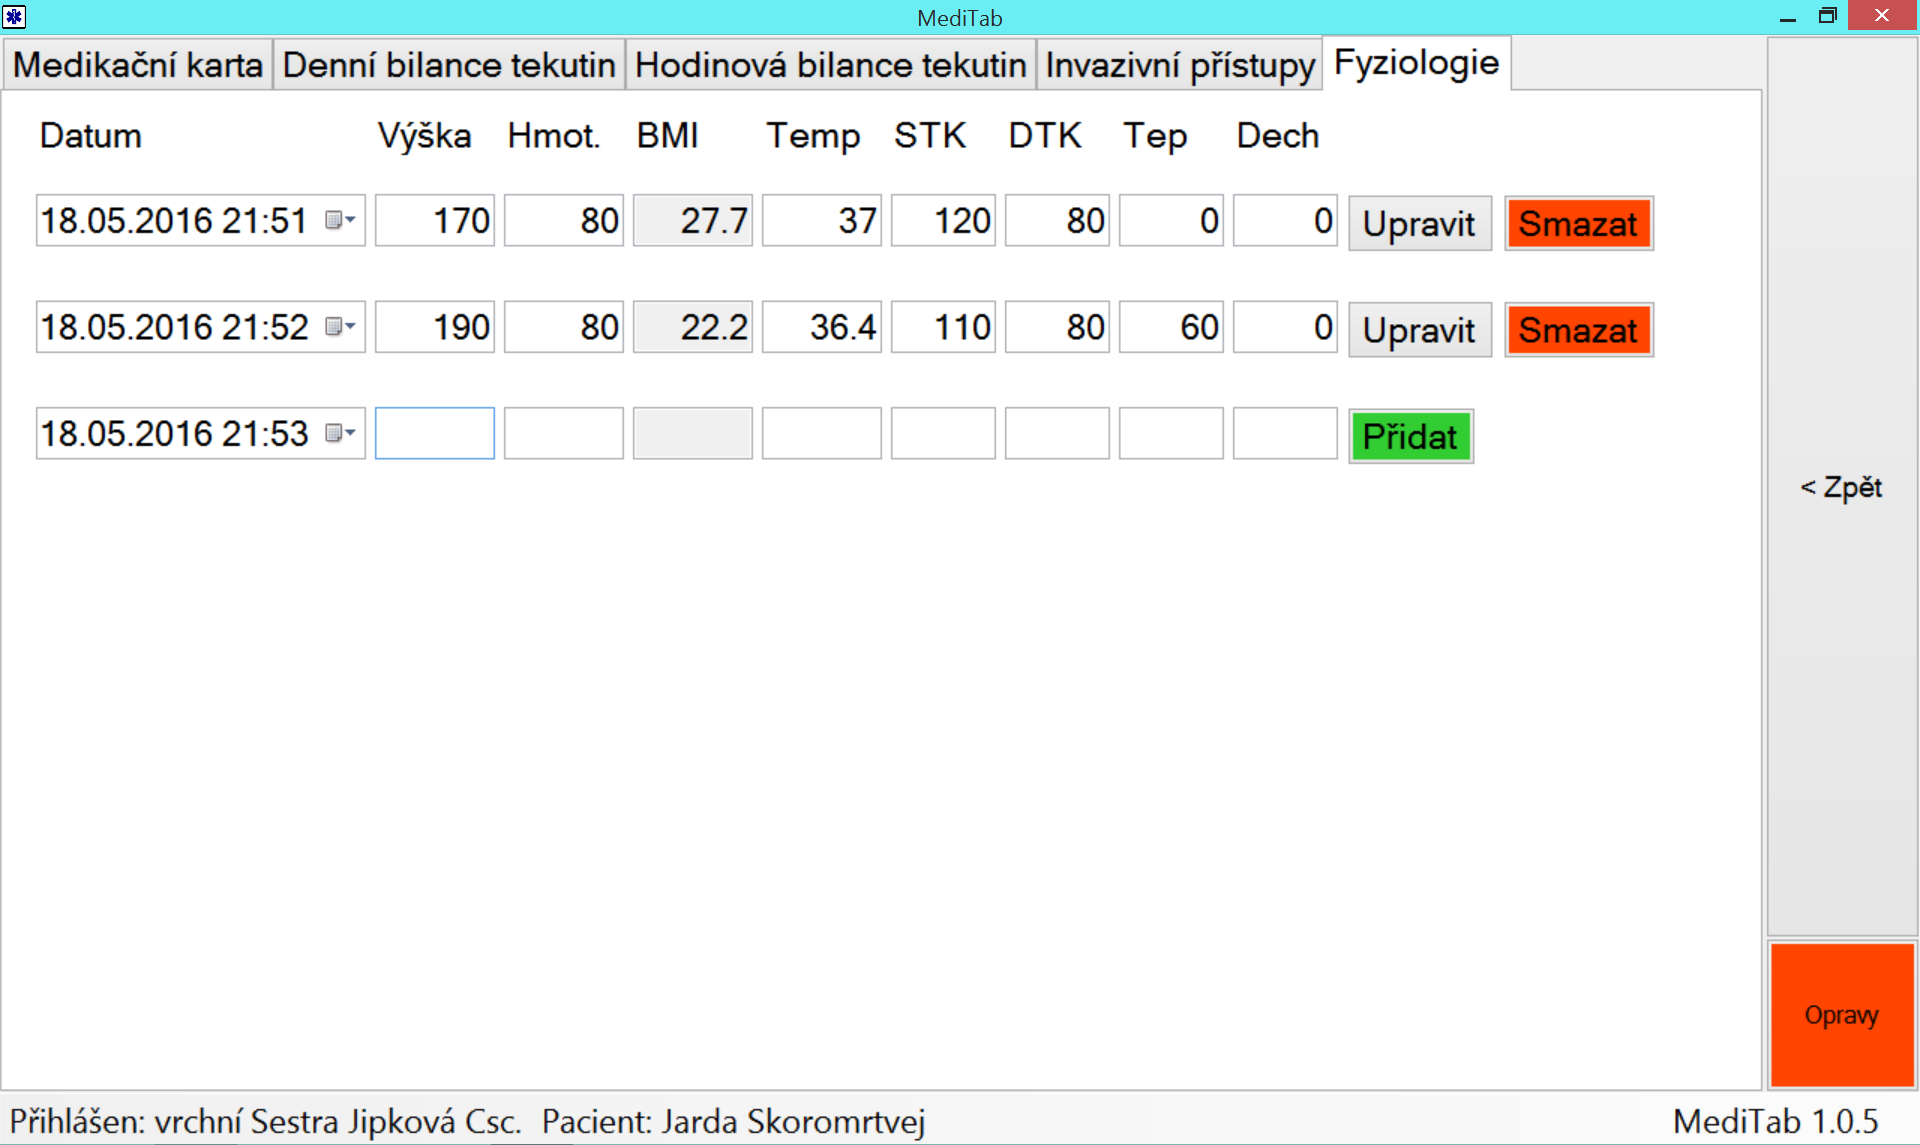
\includegraphics[width=1\textwidth]{img/meditab/fyziologie.eps}
	\caption{Fyziologie (MediTab)}
  \label{fig:fyziologie}
\end{figure}

Scrollování je opět vyřešeno pomocí MouseFilteru a TouchableFlowLayoutPanelu jako u invazivních přístupů (viz kapitola \ref{ch:pristup}).


\subsection{Opravy}

V dialogu oprav (na obrázku \ref{fig:opravy}) se zobrazují všechny akce provedené přihlášeným uživatelem na právě otevřené záložce. Každá akce je FlowLayoutPanel s časem provedení, popisem a Buttonem pro zrušení akce. Po zavření dialogu (Button \emph{Zavřít} vespod) se záložka aktualizuje.

\begin{figure}[H]
	\centering
	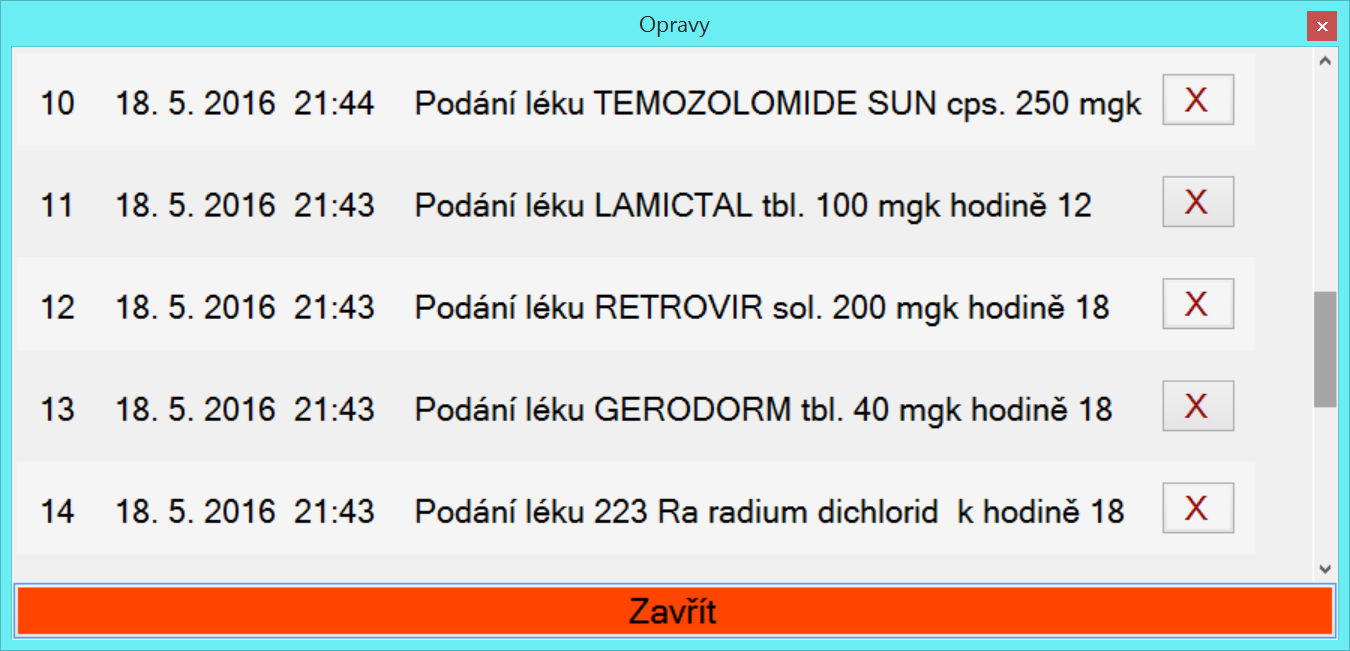
\includegraphics[width=0.8\textwidth]{img/meditab/opravy.eps}
	\caption{Opravy (MediTab)}
  \label{fig:opravy}
\end{figure}



\section{Dialogy}
\label{ch:dialogy}

Některé prvky poskytované knihovnou WinForms nejsou vhodné pro tablety. Například u MessageBoxu nelze změnit velikost písma. Proto jsem vytvořil vlastní MessageBox.

Také systémová klávesnice není optimální. Po kliknutí do textového pole se automaticky nezobrazí, ale musí se kliknout na malé tlačítko v liště. Pro numerickou klávesnici je nutné provést ještě o jeden klik navíc pro přepnutí. Při použití klávesnice často zakryla pole, do kterého se zapisovalo, a uživatel tak psal \emph{naslepo}. To v nemocnici není žádoucí a vedlo to k vytvoření vlastní klávesnice a numerické klávesnice.

\subsection{MessageBox}

Dialog MessageBoxu obsahuje TableLayoutPanel s dvěma řádky a jedním sloupcem. V prvním řádku je text zprávy, ve druhém tlačítka zarovnaná doprava. MessageBox se zobrazuje s jedním potvrzovacím Buttonem \emph{OK} (obrázek \ref{fig:bmb1}), nebo s dvěma Buttony \emph{Ano/Ne} (obrázek \ref{fig:bmb2}) a následně vrací DialogResult podle toho, na co uživatel klikl (DialogResult.Yes nebo DialogResult.No).

\begin{figure}[H]
	\centering
	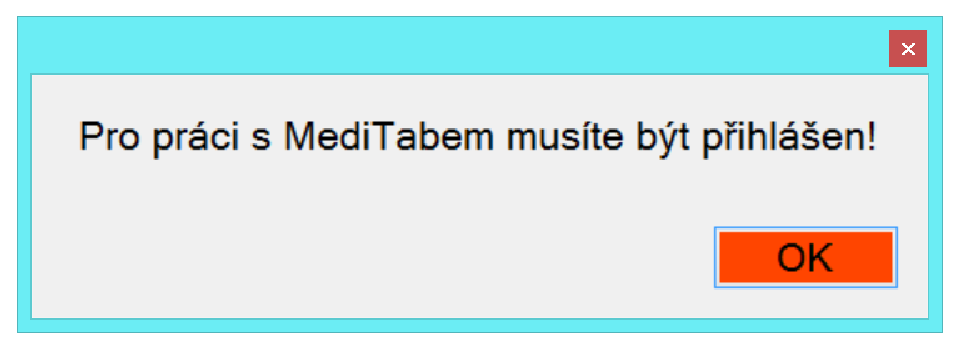
\includegraphics[width=0.5\textwidth]{img/meditab/bmb1.eps}
	\caption{MessageBox (MediTab)}
  \label{fig:bmb1}
\end{figure}

\begin{figure}[H]
	\centering
	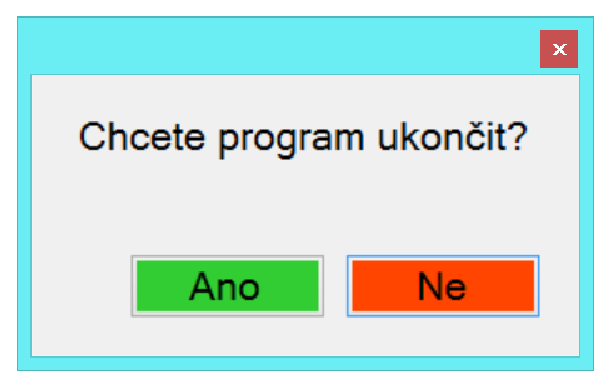
\includegraphics[width=0.3\textwidth]{img/meditab/bmb2.eps}
	\caption{MessageBox (MediTab)}
  \label{fig:bmb2}
\end{figure}

\subsection{Klávesnice}

Rozložení klávesnice odpovídá klasické klávesnici. Pro větší přehlednost neobsahuje veškeré speciální znaky, ale pouze ty, které jsou používány v nemocnici. V horní části je TextBox, ve kterém uživatel vidí, co píše (viz obrázek \ref{fig:keyboard}). Při zobrazení klávesnice může být TextBox již vyplněn textem z pole, do kterého se zapisuje. Vrací DialogResult.OK, pokud uživatel potvrdí zápis, nebo DialogResult.Cancel, pokud nepotvrdí.

\begin{figure}[H]
	\centering
	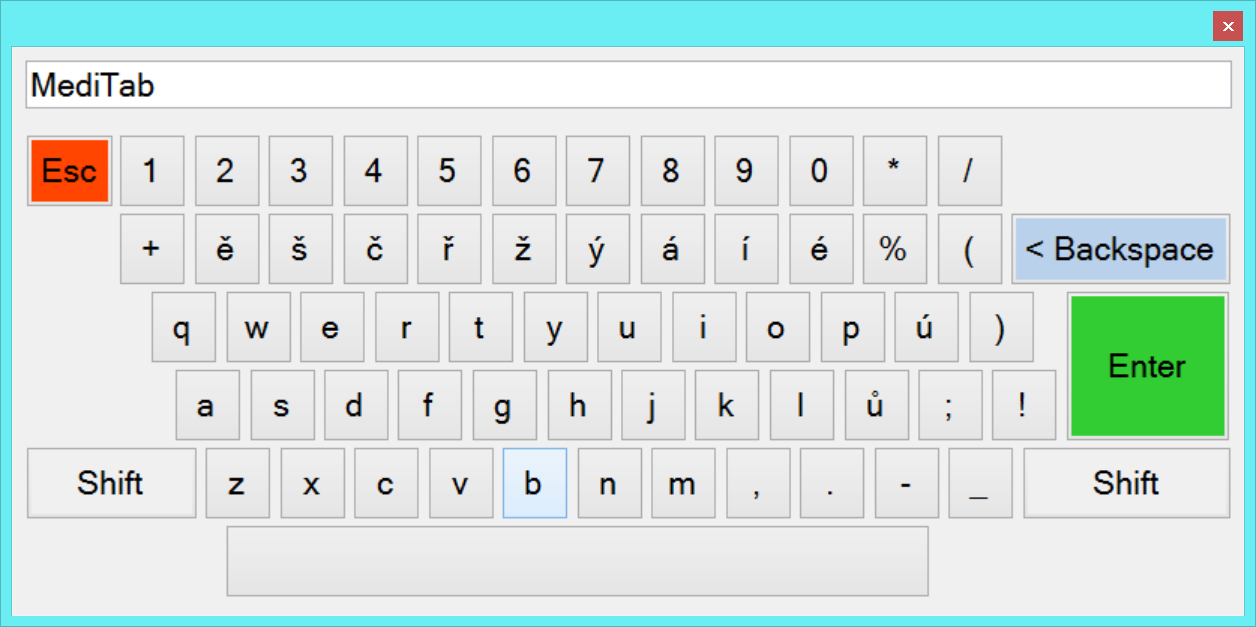
\includegraphics[width=0.8\textwidth]{img/meditab/keyboard.eps}
	\caption{Klávesnice (MediTab)}
  \label{fig:keyboard}
\end{figure}

\subsection{Numerická klávesnice}

Jednoduchá numerická klávesnice pouze s ciframi, desetinnou čárkou a potvrzovacími tlačítky (viz obrázek \ref{fig:keyboard_num}). Klávesnice má dva módy, s aktivní či neaktivní desetinnou čárkou. V horní části je TextBox stejně, jako je tomu u předešlé klávesnice. Vrací DialogResult.OK, pokud uživatel potvrdí zápis, nebo DialogResult.Cancel, pokud nepotvrdí.

\begin{figure}[H]
	\centering
	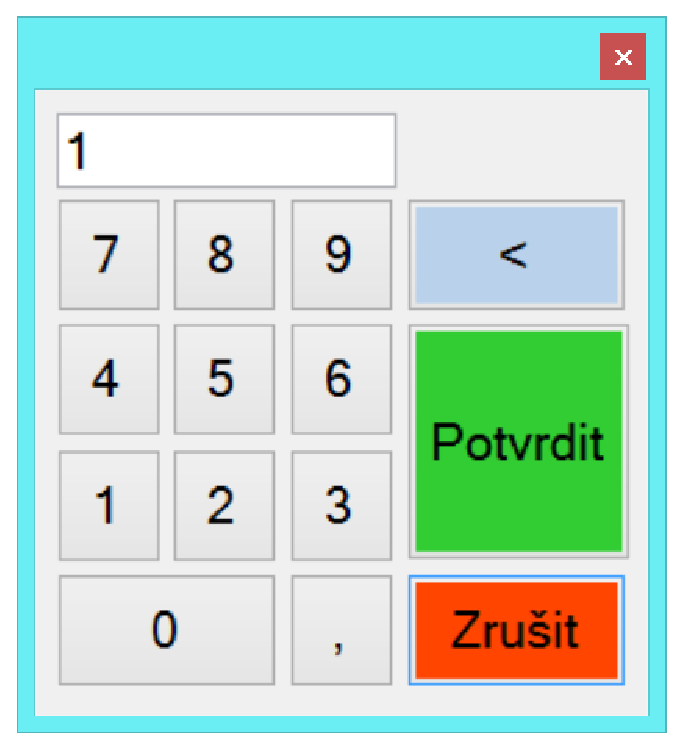
\includegraphics[width=0.3\textwidth]{img/meditab/keyboard_numeric.eps}
	\caption{Numerická klávesnice (MediTab)}
  \label{fig:keyboard_num}
\end{figure}
\chapter{Testování}
\label{ch:test}

Od aplikace je vyžadována vysoká spolehlivost. Proto musí být důkladně otestována. Testována je základní funkcionalita (tj. správné chování aplikace, konzistentnost dat v databázi) a chování při zadání nekorektních dat (data mimo povolený rozsah, data v nesprávném formátu). Testování je prováděno manuálně.

První fáze testování probíhá již při vytváření nové funkcionality. Já a~kolega \emph{Daniel Švarc}, který se podílí na vývoji aplikace (logická část a přístup do databáze), testujeme správnost nově vytvořené funkcionality a reakci na zadání nekorektních dat. Testování probíhá vyzkoušením správného chování aplikace a kontrolou dat v databázi.

Druhá fáze probíhá před vytvořením release verze. V této fázi probíhá test celé aplikace. Především je kladen důraz na otestování všech nově přidaných funkcionalit a těch částí aplikace, které jimi mohly být ovlivněny. První a~druhá fáze testování probíhá na zkušební databázi mimo FN Plzeň.

Třetí fáze probíhá na oddělení SIS\footnote{Správa informačního systému} ve FN Plzeň na jejich zkušební databázi. Testování provádí kolegové ze SIS, kteří testují především nové funkce a celkovou funkčnost aplikace.

Čtvrtou fází je pilotní provoz na JIP II. IK\footnote{Jednotka intenzivní péče II. interní kliniky} FN Plzeň. Aplikace je nasazena do ostrého provozu na reálné databázi. Zdravotní sestry testují správnost chování aplikace během běžného provozu a přívětivost uživatelského rozhraní.

První pilotní provoz proběhl v průběhu února a března 2016. Aplikaci testovalo 13 zdravotních sester JIP II. IK. Testováno bylo 8 testových scénářů: podání ordinace, nepodání ordinace, přidání nového léku, zadávání denní bilance tekutin, zadávání hodinové bilance tekutin, editace invazivního přístupu, přidání nového invazivního přístupu a oprava provedené akce.

Během pilotního provozu se zjistilo, že zadávání podání ordinací je nevyhovující. Z tohoto důvodu byl pilotní provoz pozastaven. Nově bylo požadováno zobrazení infuzí, více ordinací v jednu hodinu, a s tím kompletní změna zadávání podání ordinací. V případě, že neexistuje klinická událost, zamezení zápisu do medikační karty (dříve se načetla klinická událost z předchozího dne a data se poté zkopírovala do nové, když byla vytvořena).  Dále vznikl požadavek na přidání nové záložky \emph{Fyziologie}, zobrazování datumu u bilancí tekutin a zvýšení limitů zpětného zadávání. Během provozu bylo také zjištěno, že se některá data nezapisují do databáze správně, chybí, nebo se naopak zapisují neexistující data. Po dlouhém pátrání se zjistilo, že tyto chyby pochází z nových modulů WinMedicalcu, a byly opraveny

Druhý pilotní provoz je naplánován na červen 2016.
%\documentclass[12pt, a4paper]{report}

\usepackage[czech]{babel}
\usepackage[utf8]{inputenc}
%\usepackage[cp1250]{inputenc}
\usepackage[IL2]{fontenc}
\usepackage{anyfontsize}
\usepackage{graphicx}
\usepackage{float}
\usepackage{color}

\title{Manuál aplikace MediTab}
\author{David Pivovar}

%%%%%%%%%%%%%%%%%%%%%%%%%%%%%%%%%%%%%%%%%%%%%%%%%%%%%%%%%%%
%%%%%Makra%%%%%%%%%%%%%%%%%%%%%%%%%%%%%%%%%%%%%%%%%%%%%%%%%

% Tato makra přesvědčují mírně ošklivým trikem LaTeX, aby hlavičky kapitol
% sázel příčetněji a nevynechával nad nimi spoustu místa. Směle ignorujte.
\makeatletter
\def\@makechapterhead#1{
  {\parindent \z@ \raggedright \normalfont
   \Huge\bfseries \thechapter. #1
   \par\nobreak
   \vskip 20\p@
}}
\def\@makeschapterhead#1{
  {\parindent \z@ \raggedright \normalfont
   \Huge\bfseries #1
   \par\nobreak
   \vskip 20\p@
}}
\makeatother

% Toto makro definuje kapitolu, která není očíslovaná, ale je uvedena v obsahu.
\def\chapwithtoc#1{
\chapter*{#1}
\addcontentsline{toc}{chapter}{#1}
}



%%%%%%%%%%%%%%%%%%%%%%%%%%%%%%%%%%%%%%%%%%%%%%%%%%%%%%%%%%%
%%%%%Zacatek dokumentu%%%%%%%%%%%%%%%%%%%%%%%%%%%%%%%%%%%%%

\begin{document}

%%%%%%%%%%%%%%%%%%%%%%%%%%%%%%%%%%%%%%%%%%%%%%%%%%%%%%%%%%%
%%%%%Titulni strana%%%%%%%%%%%%%%%%%%%%%%%%%%%%%%%%%%%%%%%%
\begin{titlepage}

\begin{center}

\vspace*{50pt}
	
	{\fontsize{36}{0} \textbf{
		{\color{red}MediTab}
	}}
	
	\vfill
	
	{\fontsize{28}{0} \textbf{
		Manuál
	}}
	
	\vfill
	\vfill
	
	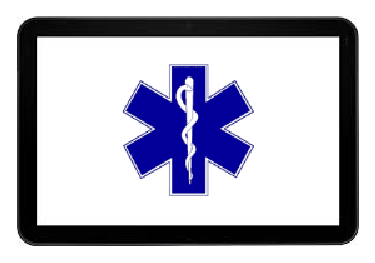
\includegraphics[width=0.7\textwidth]{img/logo_wide.eps}

\end{center}

\vspace{110pt}

\begin{flushleft}

	{\fontsize{20}{0} \selectfont
		David Pivovar\\[5pt]
		%Daniel Švarc
		\hfill
		Verze 1.0
	}
	
\end{flushleft}

\end{titlepage}


\tableofcontents

%%%%%%%%%%%%%%%%%%%%%%%%%%%%%%%%%%%%%%%%%%%%%%%%%%%%%%%%%%%
%%%%%Kapitoly%%%%%%%%%%%%%%%%%%%%%%%%%%%%%%%%%%%%%%%%%%%%%%

\chapter*{Úvod}
\addcontentsline{toc}{chapter}{Úvod}

Předmětem této práce je vytvořit grafické uživatelské rozhraní tabletové aplikace pro jednotku intenzivní péče ve Fakultní nemocnici v Plzni. Tato aplikace je určena především pro zdravotní sestry. Na nemocničním pokoji bude k dispozici tablet s aplikací, kde zdravotní sestra bude mít k dispozici aktuální data o pacientech a bude do aplikace zanamenávat své provedené úkony.

Aplikace nahradí tištěnou formu medikačních záznamů a záznamů o pacientech. Umožní tak okamžitý přístup k datům v databázi a zefektivní proces přenosu a ukládání nových aktuálních dat. Aplikace zefektivní práci jak zdravotních sester, tak i lékařů. Každý provedený úkon zdravotní sestrou se okamžitě promítne do databáze a lékař ho uvidí na svém PC. Díky propojení dat s databází se předejde ručnímu přepisování, při kterém se zvyšuje chybovost.

Cílem je vytvořit jednoduché a intuitivní uživatelské rozhraní, které se podobá zavedeným postupům ve FN Plzeň. Vzorem pro vývoj tabletové aplikace je desktopová aplikace WinMedicalc vyvíjená plzeňskou firmou Medicalc software s.r.o. ve spolupráci se SIS FN Plzeň\footnote{Správa informačního systému (IT oddělení nemocnice)}.

Tabletovou aplikaci pro jednotku intenzivní péče jsem nazval pracovním názvem \emph{MediTab}.

V první časti této práce je popsáno prostředí jednotky intenzivní péče nemocnice a aplikace WinMedicalc, části, které jsou společné s vyvíjenou aplikací (kapitola \ref{ch:fn}). Druhá část se zabývá požadavky na vyvíjenou aplikaci (kapitola \ref{ch:specifikace}) a jejím návrhem (kapitola \ref{ch:navrh}). V poslední části je popsána implementace uživatelského rozhraní (kapitola \ref{ch:implementace}) a průběh testování aplikace (kapitola \ref{ch:test}).
\chapter{Manuál}

%%%%%%%%%%%%%%%%%%%%%%%%%%%%%%%%%%%%%%%%%%%%%%%%%%%%%%%%%%%


\end{document}

%\includepdf{chapters/manual}
\setlength{\parskip}{1em}

\chapter*{Závěr}
\addcontentsline{toc}{chapter}{Závěr}

Dle zadání jsem navrhl uživatelské rozhraní tabletové aplikace pro jednotku intenzivní péče ve FN Plzeň, k čemuž jsem musel nastudovat způsob práce zdravotních sester v nemocnici, zadávání lékařských záznamu o pacientech a program WinMedicalc (části, které souvisí s vývojem aplikace). Následně jsem uživatelské rozhraní implementoval a dále vyvýjel dle připomínek SIS\footnote{Správa informačního systému} FN Plzeň a zdravotních sester. V průběhu vývoje jsem celou aplikaci průběžně testoval na správnou funkčnost. K aplikaci jsem vytvořil uživatelský manuál.

Využití informačních technologií ve zdravotnictví je široké a roste význam jejich použití. Aplikace MediTab je velkým přínosem pro nemocnici. Nadále pokračuje její vývoj a rozšiřuje se. Aktuálně je naplánován druhý pilotní provoz. V případě, že bude úspěšný, bude aplikace nasazena do ostrého provozu na více odděleních.

\listoffigures

%\begin{thebibliography}
%	\bibitem{}
%\end{thebibliography}

\chapter*{Manuál}
\addcontentsline{toc}{chapter}{Příloha: Manuál}

%%%%%%%%%%%%%%%%%%%%%%%%%%%%%%%%%%%%%%%%%%%%%%%%%%%%%%%%%%%


\end{document}
